% A LaTeX template for ARTICLE version of the MSc Thesis submissions to 
% Politecnico di Milano (PoliMi) - School of Industrial and Information Engineering
%
% S. Bonetti, A. Gruttadauria, G. Mescolini, A. Zingaro
% e-mail: template-tesi-ingind@polimi.it
%
% Last Revision: October 2021
%
% Copyright 2021 Politecnico di Milano, Italy. Inc. NC-BY

\documentclass[11pt,a4paper]{article} 

%------------------------------------------------------------------------------
%	REQUIRED PACKAGES AND  CONFIGURATIONS
%------------------------------------------------------------------------------
% PACKAGES FOR TITLES
\usepackage{titlesec}
\usepackage{color}

% PACKAGES FOR LANGUAGE AND FONT
\usepackage[utf8]{inputenc}
\usepackage[english]{babel}
\usepackage[T1]{fontenc} % Font encoding
\usepackage{amsfonts}

% PACKAGES FOR IMAGES
\usepackage{graphicx}
\graphicspath{{Images/}}
\usepackage{eso-pic} % For the background picture on the title page
\usepackage{subfig} % Numbered and caption subfigures using \subfloat
\usepackage{caption} % Coloured captions
\usepackage{transparent}

% STANDARD MATH PACKAGES
\usepackage{amsmath}
\usepackage{amsthm}
\usepackage{bm}
\usepackage[overload]{empheq}  % For braced-style systems of equations

% PACKAGES FOR TABLES
\usepackage{tabularx}
\usepackage{longtable} % tables that can span several pages
\usepackage{colortbl}

% PACKAGES FOR ALGORITHMS (PSEUDO-CODE)
\usepackage{algorithm}
\usepackage{algorithmic}

% PACKAGES FOR REFERENCES & BIBLIOGRAPHY
\usepackage[colorlinks=true,linkcolor=black,anchorcolor=black,citecolor=black,filecolor=black,menucolor=black,runcolor=black,urlcolor=black]{hyperref} % Adds clickable links at references
\usepackage{cleveref}
\usepackage[square, numbers, sort&compress]{natbib} % Square brackets, citing references with numbers, citations sorted by appearance in the text and compressed
\bibliographystyle{plain} % You may use a different style adapted to your field

% PACKAGES FOR THE APPENDIX
\usepackage{appendix}

% PACKAGES FOR ITEMIZE & ENUMERATES 
\usepackage{enumitem}

% OTHER PACKAGES
\usepackage{amsthm,thmtools,xcolor} % Coloured "Theorem"
\usepackage{comment} % Comment part of code
\usepackage{fancyhdr} % Fancy headers and footers
\usepackage{lipsum} % Insert dummy text
\usepackage{tcolorbox} % Create coloured boxes (e.g. the one for the key-words)
\usepackage{listings}
\usepackage{hyperref}
\lstset{
  language=R,
  basicstyle=\ttfamily\small, % Tipo di carattere
  %commentstyle=\color{green}, % Colore dei commenti
  %keywordstyle=\color{blue}, % Colore delle parole chiave
  %stringstyle=\color{red}, % Colore delle stringhe
  showstringspaces=false, % Mostra gli spazi nelle stringhe
  breaklines=true, % Va a capo automaticamente se una linea è troppo lunga
  breakatwhitespace=true % Va a capo solo quando ci sono spazi vuoti
}

%-------------------------------------------------------------------------
%	NEW COMMANDS DEFINED
%-------------------------------------------------------------------------
% EXAMPLES OF NEW COMMANDS -> here you see how to define new commands
\newcommand{\bea}{\begin{eqnarray}} % Shortcut for equation arrays
\newcommand{\eea}{\end{eqnarray}}
\newcommand{\e}[1]{\times 10^{#1}}  % Powers of 10 notation
\newcommand{\mathbbm}[1]{\text{\usefont{U}{bbm}{m}{n}#1}} % From mathbbm.sty
\newcommand{\pdev}[2]{\frac{\partial#1}{\partial#2}}
% NB: you can also override some existing commands with the keyword \renewcommand

%----------------------------------------------------------------------------
%	ADD YOUR PACKAGES (be careful of package interaction)
%----------------------------------------------------------------------------


%----------------------------------------------------------------------------
%	ADD YOUR DEFINITIONS AND COMMANDS (be careful of existing commands)
%----------------------------------------------------------------------------


% Do not change Configuration_files/config.tex file unless you really know what you are doing. 
% This file ends the configuration procedures (e.g. customizing commands, definition of new commands)
% Configuration package
\usepackage[bottom=2.0cm,top=2.0cm,left=2.0cm,right=2.0cm]{geometry}
\raggedbottom 

% Create color bluePoli (-> manuale grafica coordinata:  https://www.polimi.it/fileadmin/user_upload/il_Politecnico/grafica-coordinata/2015_05_11_46xy_manuale_grafica_coordinata.pdf)
\definecolor{bluePoli}{cmyk}{0.4,0.1,0,0.4}

% Custom theorem environments
\declaretheoremstyle[
  headfont=\color{bluePoli}\normalfont\bfseries,
  bodyfont=\color{black}\normalfont\itshape,
]{colored}

\captionsetup[figure]{labelfont={color=bluePoli}} % Set colour of the captions
\captionsetup[table]{labelfont={color=bluePoli}} % Set colour of the captions
\captionsetup[algorithm]{labelfont={color=bluePoli}} % Set colour of the captions

\theoremstyle{colored}
\newtheorem{theorem}{Theorem}[section]
\newtheorem{proposition}{Proposition}[section]

% Enhances the features of the standard "table" and "tabular" environments.
\newcommand\T{\rule{0pt}{2.6ex}}
\newcommand\B{\rule[-1.2ex]{0pt}{0pt}}

% Algorithm description
\newcounter{algsubstate}
\renewcommand{\thealgsubstate}{\alph{algsubstate}}
\newenvironment{algsubstates}{
    \setcounter{algsubstate}{0}%
    \renewcommand{\STATE}{%
    \stepcounter{algsubstate}%
    \Statex {\small\thealgsubstate:}\space}
    }{}
    
% Custom theorem environment
\newcolumntype{L}[1]{>{\raggedright\let\newline\\\arraybackslash\hspace{0pt}}m{#1}}
\newcolumntype{C}[1]{>{\centering\let\newline\\\arraybackslash\hspace{0pt}}m{#1}}
\newcolumntype{R}[1]{>{\raggedleft\let\newline\\\arraybackslash\hspace{0pt}}m{#1}}

% Custom itemize environment
\setlist[itemize,1]{label=$\bullet$}
\setlist[itemize,2]{label=$\circ$}
\setlist[itemize,3]{label=$-$}
\setlist{nosep}

% Create command for background pic
\newcommand\BackgroundPic{% Adding background picture
	\put(237,365){
	    \parbox[b][\paperheight]{\paperwidth}{%
	    \vfill
		\centering
		\transparent{0.4}
		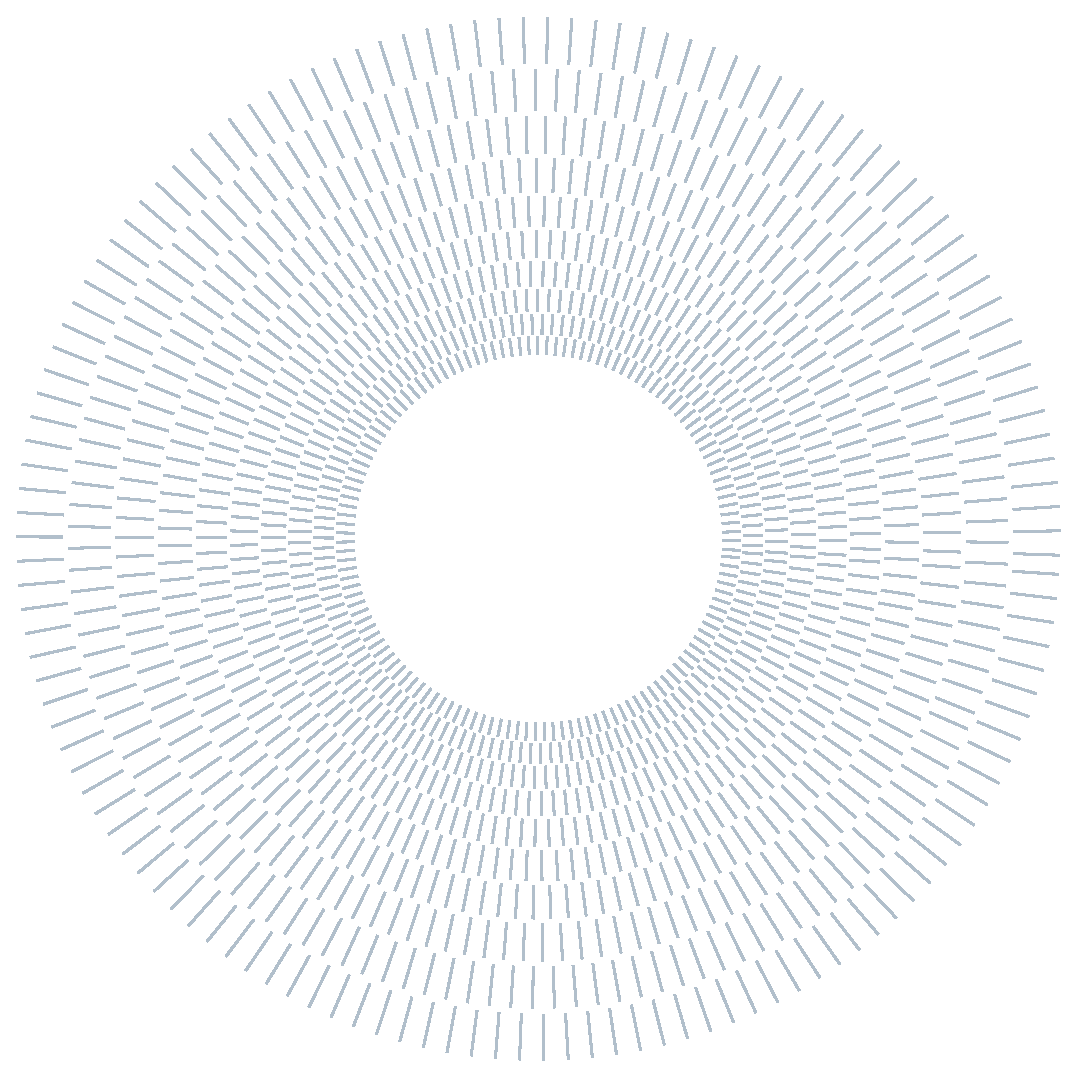
\includegraphics[width=0.44\paperwidth]{raggiera_polimi.eps}%
		\vfill}
		}
}

% Set indentation
\setlength\parindent{0pt}

% Custom title commands
\titleformat{\section}
{\color{bluePoli}\normalfont\Large\bfseries}
{\color{bluePoli}\thesection.}{1em}{}
\titlespacing*{\section}
{0pt}{3.3ex}{3.3ex}

\titleformat{\subsection}
{\color{bluePoli}\normalfont\large\bfseries}
{\color{bluePoli}\thesubsection.}{1em}{}
\titlespacing*{\subsection}
{0pt}{3.3ex}{3.3ex}

% Custom headers and footers
\pagestyle{fancy}
\fancyhf{}
      
\fancyfoot{}
\fancyfoot[C]{\thepage} % page
\renewcommand{\headrulewidth}{0mm} % headrule width
\renewcommand{\footrulewidth}{0mm} % footrule width

\makeatletter
\patchcmd{\headrule}{\hrule}{\color{black}\hrule}{}{} % headrule
\patchcmd{\footrule}{\hrule}{\color{black}\hrule}{}{} % footrule
\makeatother

% Insert here the info that will be displayed into your Title page 
% -> title of your work
\renewcommand{\title}{Ordinal Mixed-Effects Random Forest: an innovative statistical method to perform learning analytics.}
% -> author name and surname
\renewcommand{\author}{Giulia Bergonzoli}
% -> MSc course
\newcommand{\course}{Mathematical Engineering - Ingegneria Matematica}
% -> advisor name and surname
\newcommand{\advisor}{Dr. Chiara Masci}
% IF AND ONLY IF you need to modify the co-supervisors you also have to modify the file Configuration_files/title_page.tex (ONLY where it is marked)
\newcommand{\firstcoadvisor}{Dr.Ing. Lidia Rossi} % insert if any otherwise comment
%\newcommand{\secondcoadvisor}{Name Surname} % insert if any otherwise comment
% -> author ID
\newcommand{\ID}{994535}
% -> academic year
\newcommand{\YEAR}{2022-2023}
% -> abstract (only in English)
\renewcommand{\abstract}{In this work an innovative statistical method is proposed. The model is called Ordinal Mixed-Effect Random Forest (OMERF) and extends the use of random forest
to the analysis of hierarchical data to model ordinal categorical responses.
It preserves the flexibility and ability of modeling complex patterns of both categorical and continuous variables, typical of tree-based ensemble methods.
At the same time, OMERF takes into account the nested structure of hierarchical data, modeling the dependence structure that exists at the highest level of the hierarchy and allowing statistical inference on this structure.
In this study, a simulation is conducted to validate the performance of the proposed method and to compare OMERF against existing classical models.
The application of OMERF is exemplified in a case study focusing on modeling students at risk of failure from a prestigious high school in Milan, and generally on predicting their academic progress. 
The model is able to identify discriminating student characteristics and estimate the effect of each class to which students belong.}

% -> key-words (only in English)
\newcommand{\keywords}{ordinal response, hierarchical data, random forest, mixed-effects models, learning analytics}

%-------------------------------------------------------------------------
%	BEGIN OF YOUR DOCUMENT
%-------------------------------------------------------------------------
\begin{document}

%-----------------------------------------------------------------------------
% TITLE PAGE
%-----------------------------------------------------------------------------
% Do not change Configuration_files/TitlePage.tex (Modify it IF AND ONLY IF you need to add or delete the Co-advisors)
% This file creates the Title Page of the document
% DO NOT REMOVE SPACES BETWEEN LINES!

\AddToShipoutPicture*{\BackgroundPic}

\hspace{-0.6cm}
\includegraphics[width=0.6\textwidth]{logo_polimi_ing_indinf.eps}

\vspace{-1mm}
\Large{\textbf{\color{bluePoli}{\title}}}\\

\vspace{-0.2cm}
\fontsize{0.3cm}{0.5cm}\selectfont \bfseries \textsc{\color{bluePoli} Tesi di Laurea Magistrale in \\ \course}\\

\vspace{-0.2cm}
\large{\textbf{\author, \ID}}

\small \normalfont

\vspace{11pt}

\centerline{\rule{1.0\textwidth}{0.4pt}}

\begin{center}
\begin{minipage}[t]{.24\textwidth}
\begin{minipage}{.90\textwidth}
\noindent
\scriptsize{\textbf{Advisor:}} \\
\advisor \\
\\
\textbf{Co-advisors:} \\ % leave it if any co-advisor otherwise comment
\firstcoadvisor \\ % leave it if any co-advisor otherwise comment
%\secondcoadvisor \\ % leave it if you have more that one co-advisor otherwise comment (if you have more than two co-advisors just copy&paste this line writing \thirdcoadvisor, \fourthcoadvisor, ecc. (REMEMBER to modify also the main.txt)
\\ % leave it if any co-advisor otherwise comment
\textbf{Academic year:} \\
\YEAR \\
\\
\end{minipage}
\end{minipage}% This must go next to `\end{minipage}`
\begin{minipage}{.74\textwidth}
\noindent \textbf{\color{bluePoli} Abstract:} {\abstract}
\end{minipage}
\end{center}

\vspace{15pt}

\begin{tcolorbox}[arc=0pt, boxrule=0pt, colback=bluePoli!60, width=\textwidth, colupper=white]
    \textbf{Key-words:} \keywords
\end{tcolorbox}

\vspace{12pt}

\include{Thesis.tex}
%-----------------------------------------------------------------------------
% INTRODUCTION
%-----------------------------------------------------------------------------
\section{Introduction}
\label{sec:introduction}
Ordinal-scale observations are data that can be categorized into a finite and ordered set of discrete categories. However, the distances between these categories can be uneven or unknown.
\textit{"In all fields, ordinal scales result when inherently continuous variables are measured or summarized by researchers by collapsing the possible values into a set of categories. [\dots]
An ordinal variable is quantitative, however, in the sense that each level on its scale refers to a greater or smaller magnitude of a certain characteristic than another level.
Such variables are of quite a different nature than qualitative variables, which are measured on a nominal scale and have categories that do not relate to different magnitudes of a characteristic"} \cite{agresti2010analysis}.

The growing importance of ordinal categorical data shows a clear trend, driven by the increasing use of surveys and tests.
As data collection expands into various areas, there is a bigger need to model ordered data.
This type of data is usful to collect detailed information, especially in fields like market research, public opinion analysis, and healthcare, where assessing opinions, preferences, and responses is extremely important.

Ordinal classification, often known as ordinal regression \cite{mccullagh1980regression}, represents a type of multi-class classification where there is an inherent ordering relationship between the classes, but where there is not a meaningful numeric difference between them.
This type of problem occurs frequently in human created scales, which cover many domains from product reviews to medical diagnosis.

Order becomes relevant when the categories take on meanings related to strength of opinion or agreement (as in a Likert-type response) or frequency.
An explanatory example is the case where a response variable takes on four possible values: (1) strongly disagree, (2) disagree, (4) agree, (5) strongly agree. There is a natural order to the response possibilities.

This paper presents an extension of the standard random forest method \cite{breiman2001random} to ordinal data, that while investigating the learning process, takes also into account the underlying nested structure using mixed-effects models \cite{pinheiro2006mixed}.
The proposed method, called Ordinal Mixed-Effects Random Forest (OMERF), fits into the context of aggregated models.
In particular, the algorithm disentangles the estimations of fixed and random effects. It iteratively fits a random forest ignoring the grouped data structure, and a cumulative mixed-effects model based on the resultant random forest structure; a final mixed-effects random forest is reported.

In the following sections the OMERF method is described, providing a detailed description of the estimation procedure. Subsequently, two applications of the algorithm are proposed: a simulation study, comparing its performance to other existing methods, and a case study with a real world dataset.
The dataset concerns 427 students of a prestigious high school in Milan, containing  all the personal information stored in the school's electronic register.
The motivating problem of this study is to predict early and accurately the student performance, taking into account as ordinal response the final grades of the students in mathematics.
This dataset has been primarily presented in \cite{tesilidia}, nevertheless the analyses carried out in the thesis did not consider the order in the response variable and the nested data structure. Thus, we propose a more flexible and ad hoc method for the problem.

In the last few decades, learning analytics is receiving particular attention.
The primary focus lies in identifying the most effective model in terms of detecting student at risk of failure, in the context of Early Warning Systems.
\textit{"An early warning system is an intentional process whereby school personnel collectively analyze student data to monitor students at risk of falling off track for graduation and to provide the interventions and resources to intervene"} \cite{davis2013organizing}.

There is a growing interest among academics in predicting underperforming young students, driven by the potential benefits of remedial learning that align with the institution's objective of offering high-quality educational environments \cite{wilkins2016dropout}.
Furthermore, the field of data mining in education is rapidly gaining significance as it enables the discovery of valuable insights from a large amount of student data \cite{wibawa2021learning,paul2020exploring}.
A. A. Saa \cite{saa2016educational} defines \textit{"Educational Data Mining (EDM) is a new trend in the data mining and Knowledge Discovery in Databases (KDD) field
which focuses in mining useful patterns and discovering useful knowledge from the educational information systems [\dots]. Researchers in this field
focus on discovering useful knowledge either to help the educational institutes manage their students better, or to help students to manage their education and deliverables better and
enhance their performance"}.


Results reveal that in a nonlinear setting the proposed method performs better or comparably with respect to existing models; providing substantial improvements and having the advantages of increasing the knowledge about the multilevel nature of data and their complex dependencies.

Section \ref{sec:literature_rev} conducts a review of the existing literature related to methods analogous to the one proposed. Section \ref{sec:methods} articulates the OMERF method, outlining its theoretical foundations and its implementation.  Section \ref{sec:sim} is intended
for the description of a simulation study. Section \ref{sec:case} delves into the details of the previously mentioned case study. Ultimately,  Section \ref{sec:conclusions} is dedicated to highlighting conclusions and fostering a discussion.

All the analysis are performed using R software \cite{rlanguage} and all the R codes for the OMERF algorithm and for both simulation and case study are available in the following github repository: \url{https://github.com/giuliabergonzoli/Master_Thesis}.

\section{Literature review}
\label{sec:literature_rev}
The method proposed in this study takes inspiration from the so-called aggregated methods.
These methods refer to that type of algorithms which focus on incorporating tree-based approaches \cite{breiman2017classification}, or their ensembles (like random forest \cite{breiman2001random}), into mixed-effects models \cite{pinheiro2006mixed}.
Tree-based models are increasingly popular for their ability to capture complex and nonlinear relationships; this combination with mixed models allows their extension to the analysis of both nested and longitudinal data. The first are data that present a hierarchical multilevel structure, the second refer to the situation where repeated observations are available for each sampled object.

It is important to account for this framework, as it can provide significant insights that might otherwise be neglected, enabling the quantification of the portion of variability in the response variable that is attributable to each level of grouping. Nested data are not independently and identically distributed (i.i.d) as in classical regression and classification models, but their distribution depend on their grouping structure.
Analysing and disentangling the effects associated with each level of the hierarchy enables a deeper understanding and investigation of the latent structure present at the highest level of the hierarchy, thereby increasing the comprehension of the phenomenon described by the data.

Aggregated methods developed in statistical literature can be categorized into two groups: the first that focuses on Gaussian responses, making it unsuitable for classification tasks, while the second group extends its applicability to non-Gaussian data and is suitable for addressing classification problems.

The works in \cite{sela2012re,hajjem2011mixed,hajjem2014mixed} pertains to the first collection of models.
In the work of Sela and Simonoff \cite{sela2012re}, it is implemented the Random Effects Expectation-Maximization (RE-EM) tree; while in \cite{hajjem2011mixed} Hajjem et al. propose the Mixed-Effect Regression Tree (MERT) model.
They both are extensions of a conventional regression tree to account for clustered and longitudinal data, sobstituting the linear fixed part of a linear mixed effects model with the tree estimates. 
Then, trying to improve prediction accuracy, in \cite{hajjem2014mixed} the authors replace the regression tree with a random forest, introducing a method known as Mixed-Effects Random Forest (MERF).

With regard to the extension to other types of outcomes, in \cite{hajjem2017generalized} the linear structure used to model the fixed effects component in a generalized linear mixed model's predictor is replaced with a regression tree structure, obtaining the Generalized Mixed-Effects Regression Tree (GMERT), which is basically the MERT approach extended to non-Gaussian responses.
Another expansion of a classification problem is the introduction of the Generalized Mixed-Effects Tree (GMET) \cite{fontana2021performing}. It starts by initialising the random-effects to zero, then it estimates the target variable through a generalized linear model, builds a regression tree using
the estimated target variable as the dependent variable and finally fits a mixed-effects model to estimate the random-effects part, using the fixed-effects part estimated by the tree as an offset.
In \cite{fokkema2018detecting}, the authors propose an algorithm known as Generalized Linear Mixed-effects Model tree (GLMM tree), which iteratively refines the estimates of a generalized linear model tree and a mixed-effects model until convergence is achieved.
Lastly, in \cite{speiser2020bimm}, the authors introduce a decision tree method for modeling clustered and longitudinal binary outcomes within a Bayesian framework, called Binary Mixed Model tree (BiMM tree).

Another step forward in the field of tree-based aggregated models has been done by Pellagatti et al. in \cite{pellagatti2021generalized}, implementing the Generalized Mixed-Effects Random Forest (GMERF) and thus extending for the first time random forest, and not only simple trees, to deal with hierarchical data, both for regression and classification (for any response variable in the exponential family).

To integrate into this existing literature and contribute an additional step, the current research work proposes a novel method called Ordinal Mixed-Effects Random Forest (OMERF), that is inspired by the GMERF model, but extends the random forest to deal with ordinal data, namely, with ordinal regression problems.

Concerning the statistical literature about ordinal data, one of the early contributions to classification techniques for ordinal data can be found in \cite{mccullagh1980regression}, where a regression model is introduced. Its multilevel extention, the random effects cumulative model, is described in \cite{tutz1996random}, where ordinal regression models as special cases of multivariate generalized linear models are extended to include random effects in the linear predictor.

With regard to the implementation of nonlinear ordinal models, some attempts to implement new techniques can be found in the literature.
The work in \cite{tutz2003generalized} proposes an extension of ordinal regression through the generalization of the additive model by incorporating nonparametric terms; in \cite{shashua2002ranking} Shashua and Levin introduce a generalised formulation for the support vector machine for ordinal data; finally, the ordinal random forest method is presented in \cite{hornung2020ordinal}, which is a random forest-based prediction method for ordinal response variables.

Nonetheless, to the best of our knowledge, this is the first time that random forest is extended to deal with both the ordinal classification setting and nested structures, implementing an ordinal model which is able to capture complex nonlinear data relationships, and at the same time to inspect and understand the multilevel nature of data.


%-----------------------------------------------------------------------------
% EQUATIONS
%-----------------------------------------------------------------------------
\section{Model and Methods}
\label{sec:methods}
In this section, a concise overview of cumulative link models for ordinal categorical data (Section \ref{sec:clm} and \ref{sec:clmm}) and random forest (Section \ref{sec:rf}) is provided.
This will serve as the foundation for the explanation and understanding of the OMERF method and its algorithm detailed in Section \ref{sec:omerf}.  Section \ref{sec:gof} is devoted to inspect different performance measures to evaluate the Goodness of Fit of ordinal models.
These measures serve as assessment criteria for the compared models.

\subsection{Background and state of the art models}

\subsubsection{Cumulative link models}
\label{sec:clm}
A Cumulative Link Model (CLM) \cite{agresti2010analysis,ananth1997regression,mccullagh1980regression} is an analytical framework to deal with observations on an ordinal scale.
These models applied to ordinal responses are advantageous in the fact that there is no need to define interval-scale assumptions about distances between response categories.

Ordinal observations can be expressed through a random variable, \(y_{j}\), which takes on the value \(c\) when the \(j\)-th ordinal observation falls within the \(c\)-th category. \(c\) takes integer values in the range from 1 to \(C\), where \(C\) is greater than or equal to 2.

The linear predictor of CLMs can be expressed as follows:
\begin{equation}
    \label{clm}
    \begin{aligned}
        \eta_{jc} &= g(\gamma_{jc}) = \theta_{c} - \bm{x}_{j}^T \bm{\beta}, \qquad  j=1,\dots,J \qquad c=1,\dots,C-1
    \end{aligned}
\end{equation}
where \(\gamma_{jc} = \mathbb{P}(y_{j} \leq c) = \pi_{j1} + \dots + \pi_{jc}\) (with \(\sum_{c=1}^{C} \pi_{jc}=1\)) are cumulative probabilities, \(\pi_{jc}\) is the probability that the \(j\)-th observation falls in the \(c\)-th category, \(\eta_{jc}\) is the linear predictor
and \(\bm{x}_{j}\) is a \(p\)-dimensional vector of fixed effects regression variables, to which corresponds the parameter vector \(\bm{\beta}\).
Finally, \(g\) is the monotonic, differentiable link function and \(\theta_{c}\) are the strictly ordered thresholds (also known as cut-points or intercepts):
\begin{gather*}
    \begin{aligned}
        -\infty \equiv \theta_{0} \leq \theta_{1} \leq \dots \leq \theta_{C-1} \leq \theta_{C} \equiv \infty.
    \end{aligned}
\end{gather*}


\subsubsection{Cumulative link mixed models}
\label{sec:clmm}
Cumulative Link Mixed Models (CLMM) \cite{grilli2011multilevel,tutz1996random} are the multilevel extension of cumulative regression models with normally distributed random effects for ordinal responses. These models are suited to handle data with a hierarchical structure: given \(\bm{y}_{i}\) = \(y_{i1}, \dots, y_{in_{i}}\) the \(n_{i}\)-dimensional response vector for observations in the \(i\)-th group, its elements \(y_{ij}\) are supposed to be conditionally independent on the random effects \(\bm{b}_{i}\).
The standard assumption on the random effects \(\bm{b}_{i}\) is that, conditionally on the fixed covariates, they are independent and identically distributed with zero mean and a common cluster covariance matrix \(\bm{\Sigma_{b}}\).
The key part of this standard assumption is the exogeneity, namely the mean of the random effects does not depend on the fixed covariates: \(\mathbb{E}(\bm{b}_{i}|\bm{x}_{ij}:j=1,\dots,n_{i})=0\).

The configuration with a random intercept and \(q\) random slopes in a two-level hierarchy can be written as:
\begin{equation}
    \label{clmm}
    \begin{aligned}
        \eta_{ijc} = g(\gamma_{ijc}) &= \theta_{c} - (\bm{x}_{ij}^T \bm{\beta} + \bm{z}_{ij}^T \bm{b}_{i}),\qquad c=1,\dots,C-1 \\
        \bm{b}_{i} &\sim \mathcal{N}_q(\bm{0},\bm{\Sigma_{b}})
    \end{aligned}
\end{equation}
where $i=1,\dots,I$ is the level 2 (group) index and $j=1,\dots,n_{i}$ (with \(\sum_{i=1}^{I} n_{i}=J\)) is the nested level 1 index, $\gamma_{ijc} = \mathbb{P}(y_{ij} \leq c)$ is the cumulative probability up to the \textit{c}-th category for unit \textit{j} in group \textit{i}.
Fixed effects are identified by parameters \(\bm{\beta}\) associated to the entire population, while random ones are identified by group-specific parameters \(\bm{b}_{i}\).
%Since the overall intercept is fixed to zero, if it is the case of a single random intercept and no random slopes, the random effect $b_{0i}$ representing unobserved factors at the cluster level, can be seen as a random shift of the threshold parameters \(\theta_{c}\) so that the set of thresholds of cluster \(i\) is \(\theta_{c}-b_{0i}\).

In cumulative link mixed models the ordinal response variable \(y_{ij}\) with \(C\) categories is generated by a latent continuous variable \(y^*_{ij}\)  with a set of \(C-1\) thresholds \(\theta^*_{c}\) such that \(y_{ij}=c\) if and only if \(\theta^*_{c-1} \leq y^*_{ij} \leq \theta^*_{c}\).
The latent continuous variable is modelled as:
\begin{equation}
    \label{cont_clmm}
    \begin{aligned}
        y^*_{ij} = \bm{x}^{T}_{ij} \bm{\beta^*} + \bm{z}_{ij}^T \bm{b}^*_{i} + \epsilon^*_{ij}
    \end{aligned}
\end{equation}
where \(\epsilon^*_{ij}\) is a level 1 error with standard deviation \(\sigma_{\epsilon^*}\).

Therefore, the cumulative probabilities are \(\gamma_{ijc} = \mathbb{P}(y_{ij} \leq c) = \mathbb{P}(y^*_{ij} \leq \theta^*_{c}) = \mathbb{P}(\epsilon^*_{ij} \leq \theta^*_{c} - \bm{x}^{T}_{ij} \bm{\beta^*} - \bm{z}_{ij}^T \bm{b}^*_{i}) = g^{-1}(\theta_{c} - \bm{x}^{T}_{ij} \bm{\beta} - \bm{z}_{ij}^T \bm{b}_{i})\).
The underlying linear model \eqref{cont_clmm} with thresholds \(\theta^*_{c}\) and level 1 error \(\epsilon^*_{ij}\) having distribution function \(g^{-1}\) is equivalent to the cumulative model \eqref{clmm} with link function \(g\).
A generic parameter \(\alpha\) of the cumulative model can be retrieved as \(\alpha = \alpha^* \frac{\sigma_{g}}{\sigma_{\epsilon^*}}\), where \(\sigma_{g}\) is the standard deviation of the distribution associated to the link function \(g\).

As explained in \cite{grilli2011multilevel}, in a linear model like the underlying continuous model \eqref{cont_clmm} the level of unobserved heterogeneity due
to the grouping of the units is summarized by the Intraclass Correlation Coefficient (ICC)
\(\rho=\sigma^2_{b_i^*}/(\sigma^2_{b_i^*}+\sigma^2_{e^*})\). In a linear model the ICC is both the proportion of the
between-group variance with respect to the total variance and the correlation between
the responses of two units of the same group, namely \(\rho = Cor(y_{ij}^*,y_{i'j}^*|x_{ij},x_{i'j})\).
Such a correlation does not depend on the covariates, so the ICC is an
exhaustive indicator of the degree of correlation. Unfortunately, this property does not hold
in models for categorical responses such as the cumulative model in \eqref{clmm}
since \(Cor(y_{ij},y_{i'j}|x_{ij},x_{i'j})\) actually depends on the covariates. A solution is to
summarize the degree of within-group correlation using the ICC for the underlying linear
model, which can be easily computed using the random group variance \(\sigma^2_{b_i}\) of the cumulative model:
in fact, from the relationship \(\sigma_{b_i} = \sigma_{b_i^*} \frac{\sigma_{g}}{\sigma_{\epsilon^*}}\), it follows that \(\rho=\sigma^2_{b_i}/(\sigma^2_{b_i}+\sigma^2_{g})\), where \(\sigma^2_{g}\)
is the variance of the distribution associated to the link function (\(\pi^2 / 3 \cong 3.29\) for the logit link function).
% However, the ICC for the underlying linear model is misleading if one attempts to compare it with the
% values usually obtained in linear models for observed continuous responses: in fact, the
% ICC for the underlying linear model is much lower and it often gives the impression of
% a negligible within-cluster correlation. For example, a value \(\rho\) = 0,01 is negligible for an
% observed response but not for an underlying response.

In the context of CLMMs, model parameters are typically estimated using maximum likelihood methods, employing techniques such as Adaptive Gaussian Quadrature, Gauss-Hermite Quadrature, or Laplace approximation to the likelihood function.
A Newton-Raphson algorithm updates the conditional modes of the random effects for the subsequent approximations and finally a nonlinear optimization is performed over the fixed parameter set to get the Maximum Likelihood Estimation.

\subsubsection{Random forest}
\label{sec:rf}
Random forest are a powerful machine learning algorithm that combines the predictive power of multiple decision trees to make accurate and robust predictions.
In particular, random forest for regression \cite{breiman2001random,james2013introduction} are tree-based ensemble methods formed by growing regression trees such that the tree predictor \(f(\bm{x})\) takes on numerical values, and the random forest predictor is formed by taking the average over \(K\) of these trees \(f_k(\bm{x})\), \(k=1,\dots,K\).
Regression trees are an extension of classification trees, in which the dependent variable is a continuous variable, and the measure of impurity is the Mean Squared Error of the observations in the node.

As in bagging, RFs build a large number of decision trees on bootstrapped training samples, independently drawn from the distribution of the random vector (\(\bm{y}\), \(\bm{X}\)), where \(\bm{y}\) is the response variable and \(\bm{X}\) are the covariates. However, when building these decision trees, each time a split in a tree is considered, a random subsample of
covariates is chosen as split candidates among the \(p\) available ones.
Ideed, at each split the algorithm considers only a subset of the available predictors in order to avoid the case in which there is a single strong predictor which will influence all the predictions and consequently, all of the bagged trees will look quite similar to each other.
This process can be thought of as decorrelating the trees, thereby making the average of the resulting trees less variable and hence more reliable.

Random forests are recently increasing in popularity for their ability to capture a more complex and nonlinear structure of the relationship between covariates and response. 
Moreover, their additional benefit is the possibility to assess the importance of features by using out-of-bag errors. This involves measuring the scaled difference in performance between models that include the variable of interest and those that do not.
However, a drawbacks of RFs compared to simple tree-based methods is their low level of interpretability.

\subsection{Ordinal mixed-effects random forest}
\label{sec:omerf}
The proposed statistical method, called Ordinal Mixed-Effects Random Forest (OMERF), extends the use of random forest to the analysis of hierarchical data, for categorical ordinal response variables.
It essentially models the fixed effects through a random forest, combining them to the random effects obtained using a CLMM, in order to take into account both possible complex functional forms of the covariates and the nested structure of data.
The method can be formulated as follow:
\begin{equation}
    \label{eq:omerf}
    \begin{aligned}
        \eta_{ijc}  = g(\gamma_{ijc}) &= \theta_{c} - (f(\bm{x}_{ij}) + \bm{z}_{ij}^T \bm{b}_{i})\\
        g(\gamma_{ijc}) = logi&t(\gamma_{ijc}) = ln(\frac{\gamma_{ijc}}{\gamma_{ijc}-1}) \\
        \gamma_{ijc} &= \mathbb{P}(y_{ij} \leq c) \\
        \bm{b}_{i} &\sim \mathcal{N}_q(\bm{0},\bm{\Sigma_{b}}) \\
        j=1,\dots,n_{i} \qquad i&=1,\dots,I \qquad c=1,\dots,C-1
    \end{aligned}
\end{equation}
where \(f(\bm{x}_{ij})\) is the unknown and nonlinear structure estimated through the random forest,
\(\gamma_{ijc}\) are cumulative probabilities, \(\pi_{ijc} = \mathbb{P}(y_{ij}=c) = \mathbb{P}(y_{ij} \leq c) - \mathbb{P}(y_{ij} \leq c-1) = logit^{-1}(\theta_{c} - (f(\bm{x}_{ij}) + \bm{z}_{ij}^T \bm{b}_{i})) - logit^{-1}(\theta_{c-1} - (f(\bm{x}_{ij}) + \bm{z}_{ij}^T \bm{b}_{i}))\) is the probability that the \(j\)-th observation, within the \(i\)-th group, falls in the \(c\)-th category and \(\eta_{ijc}\) is the linear predictor.
Similarly to CLMM model, OMERF model, assumes that the random effects \(\bm{b}_i\) and \(\bm{b}_{i'}\) are independent for \(i \neq i'\).
Fixed effects are estimated using a nonparametric RF model that concerns the entire population, while random effects are identified through group-specific parameters.

To implement the OMERF model, one must separate the estimation of the fixed and random effects components and alternate between them until convergence.
To achieve this, it can be observed that if the random effects are known in advance, a RF could be fitted to estimate the fixed part \(f(\bm{x}_{ij})\) by using \(\eta_{ijc}\) and \(\bm{b}_i\) as dependent variables.
Similarly, if the population-level effects are known, the random effects could be estimated using a cumulative link mixed-effects model with the response corresponding to \(\eta_{ijc}\) and \(f(\bm{x}_{ij})\).
Since neither of them is known, it is employed an iterative approach that alternates between estimating the RF for the fixed effects part and estimating the CLMM model for the random ones.
Convergence is considered achieved when the difference between the random effects estimates in two consecutive iterations is less than a predetermined tolerance.

Another significant consideration to address is the fact that \(\eta_{ijc}\) remains unknown and cannot be inferred directly from the available data.
To tackle this aspect, the approach, consistent with the methodology introduced in \cite{fontana2021performing,pellagatti2021generalized}, involves estimating \(\eta_{ijc}\) by employing a conventional CLM model, with the fixed effects covariates as predictors.
The pseudo-code outlining this estimation process is provided in Algorithm \ref{alg:alg_omerf}.

The random forest model is constructed using the R package \(randomForest\) \cite{RF}, which implements the original algorithm described in \cite{breiman2001random}. Meanwhile, the CLMM is built using the \(clmm\) function from the R package \(ordinal\) \cite{ordinal}.
The CLMM model allows for different offsets in the formula and scale effects, which are considered as components of the linear predictor that are known in advance and thus  they require no parameter to be estimated from the data. The implemented method in particular will make use of an offset modelled as:
\begin{equation}
    \label{scale_eff}
    \begin{aligned}
        \eta_{ijc}  &= g(\gamma_{ijc}) = \theta_{c} - \bm{z}_{ij}^T \bm{b}_{i} - offset_{ij}, \qquad  j=1,\dots,n_{i} \qquad i&=1,\dots,I \qquad c=1,\dots,C-1
    \end{aligned}
\end{equation}
where \(offset_{ij}\) =  \(f(\bm{x}_{ij})\), i.e. the random forest estimates of the fixed effects part.

To make predictions for a new observation \([\bm{x}_{ij};\bm{z}_{ij}]\), the following formula is employed: \(\hat{\eta}_{ijc} = \hat{\theta}_{c} - (\hat{f}(\bm{x}_{ij}) + \bm{z}_{ij}^T \hat{b}_{i})\).
Here, \(\hat{f}\) represents the random forest model estimated by the algorithm, \(\hat{b}_i\) is the vector of random effects coefficients associated with the \(i\)-th group, and \(\hat{\theta}_{c}\) is the threshold associated to the predicted category.


All the analysis are performed using R software \cite{rlanguage}. The R code for the OMERF algorithm and its auxiliary functions are available in Appendix \(\textcolor{red}{\ref{sec:appA}}\).

\subsection{Goodness of Fit indices for ordinal models}
\label{sec:gof}
The role of performance measures in predictive models is crucial, as they allow for the assessment of their Goodness of Fit and for the selection of the optimal model.
However, the choice of appropriate metrics for ordinal models is not straightforward and is an area of research still not widely explored.

Considering the accuracy for ordinal response outputs, it allows computing the percentage of observations correctly classified without taking into account their ordered scale, as it is typically used for classification models.
However, in our evaluations, we still find it useful to report this index's value. It is in fact an immediate, easy-to-understand measure that allows to actually see how many correct classifications have been made.
Given a set of \(y_{j}, \, j=1,\dots,N\) observed target values and  \(\hat{y}_{j}, \, j=1,\dots,N\) predicted target values, it is defined as:
\begin{equation}
    \label{eq:Acc}
    \begin{aligned}
        Accuracy=\frac{1}{N} \sum_{j=1}^{N} \mathbbm{1}_{y_{j}=\hat{y}_{j}} \quad \in [0,1]
    \end{aligned}
\end{equation}

Due to limitations highlighted regarding the accuracy measure, alternative metrics better suited for ordinal responses are being considered.
Firstly, we take into consideration Mean Square Error (defined in Equation \eqref{eq:MSE}), that accounts for the severity of the errors \cite{gaudette2009evaluation}. Indeed, in this type of scenario, some errors are worse than others.
A classifier which makes many small errors could be preferable to a classifier that makes fewer errors overall, but larger. For this reason, MSE can add meaningful infromation to the accuracy values.
\begin{equation}
    \label{eq:MSE}
    \begin{aligned}
        MSE=\frac{1}{N} \sum_{j=1}^{N} (y_{j}-\hat{y}_{j})^2 \quad \in [0,+\infty)
    \end{aligned}
\end{equation}

Furthermore, we incorporate the evaluation of two indexes that assess the similarity between two classifications of the same objects by quantifying the agreement proportions between the two partitions.  These two indices are the Adjusted Rand Index \cite{hubert1985comparing} and Cohen's kappa \cite{cohen1960coefficient}.
Both of these indices have a range from -1 to 1. Positive values in this range indicate agreement between the two sets, with 1 denoting perfect agreement. Negative values imply some degree of disagreement, and the magnitude of the negative value reflects the extent of this disagreement. A value equal to 0 suggests that the agreement is no different from what would be expected by chance.

Nevertheless, we wanted to compare the tested models with more task-specific performance measures. Thus, we select among the recent developements in the field the two indexes implemented by J. S. Cardoso \cite{cardoso2011measuring} and E. Ballante \cite{ballante2022new}.

Let consider the following quantities:
\begin{itemize}
    \item \(n_{r,c}, \, r,c=1,\dots,C\): number of points from the \(r\)-th class predicted as being from \(c\)-th class;
    \item \(Non-Discordant \, Pairs\): pairs of points \(x_{i}\) and \(x_{j}\) with sign(\((r_{x_{i}} - r_{x_{j}}) \times (c_{x_{i}} - c_{x_{j}}) \)) \(\leq 0\), where \(r_{x_{i}}\) and \(c_{x_{i}}\) are the row and column in the Confusion Matrix corresponding to \(x_{i}\), respectively;
    \item \(path\): sequence of entries in the Confusion Matrix where two consecutive entries in the path are 8-adjacent neighbours;
    \item \(consistent \, path\): \(path\) in which every pair of nodes in the path is non-discordant;
    \item \(Path\): set of all \(consistent \, paths\) in the Confusion Matrix from (1,1) to (C,C).
\end{itemize}
The index proposed by Cardoso is defined as: 
\begin{equation}
    \label{eq:OC}
    \begin{aligned}
        OC_{\beta}^{\gamma}= \min \left\{ 1 - \frac{\sum_{(r,c) \in Path} n_{r,c}}{N+(\sum_{\forall (r,c)} n_{r,c} |r-c|^{\gamma})^{1/\gamma}} + \beta \sum_{(r,c) \in Path} n_{r,c} |r-c|^{\gamma} \right\}
    \end{aligned}
\end{equation}
where \(OC_{\beta}^{\gamma} \in [0,1]\), and \(OC_{\beta}^{\gamma}=0\) if and only if all the elements of the vectors generating the Confusion Matrix are equal.

Whereas, having these definitions:
\begin{itemize}
    \item \(Classification \, function\): Let observations \(\left\{ 1,\dots, N\right\}\) be grouped by the estimated classes \(\hat{y}_{j}=c, \, j=1,\dots,N, c=1,\dots,C\). For each class, sort the observations in a non-increasing order with respect to \(p_{j,c}=\mathbb{P}(\hat{y}_{j}=c)\).
    The vector of indexes \(j\) of the observations is a permutation of the original vector, according to the ordering defined above. For a given model, the classification function is a piecewise constant function \(f_{mod}:[0,1] \rightarrow \left\{ 1,\dots, C\right\} \)
    such that \(f_{mod}([\frac{j-1}{N},\frac{j}{N}])=y_j, \, j=1,\dots,N\). As a special case, the \(perfect\) \(classification\) \(function\), is a piecewise constant function \(f_{exact}:[0,1] \rightarrow \left\{ 1,\dots, C\right\} \) such that each estimated class corresponds to the real
    class identified by \(\bm{y}\);
    \item \(Error \, Interval\): Consider the vector of observations ordered as described in the previous definition. Suppose that the range corresponding to the estimated class \(c\) in that vector has indexes in \([n_{c-1}, n_c)\). Let \(\widetilde{j}_c=n_{c-1},\dots, n_c\) be the index of the first misclassified observation.
    The error interval is defined as \([\frac{\widetilde{j}_c}{N},\frac{n_c}{N})\), i.e. the interval between the first misclassified observation and the last observation of the estimated class \(c\); its length is defined as \(e_c = \frac{n_c - \widetilde{j}_c}{N}\).
    If no misclassification occurs in \([n_{c-1}, n_c)\), the error interval is defined as an empty set with a length \(e_c\) = 0.
    Moreover, for each class \(c=1,\dots,C\) the corresponding weight \(w_c=\frac{e_c}{l_c}\), where \(e_c\) is the \(c\)-th error interval length and \(l_c=n_c-n_{c-1}\) is the length of the \(c\)-th estimated class in the domain, such that \(0 \leq w_c \leq 1\).
\end{itemize}
The index constructed by Ballante can be expressed as:
\begin{equation}
    \label{eq:Ball}
    \begin{aligned}
        I = \sum_{c=1}^{C} w_{c} \int_{\frac{n_{c-1}}{N}}^{\frac{n_{c}}{N}} |f_{mod}(x)-f_{exact}(x)|dx
    \end{aligned}
\end{equation}
where \(I \in [0,C-1]\), and \(I = 0\) if and only if \(f_{mod} = f_{exact}\).

Its normalized version is:
\begin{equation}
    \label{eq:Ball}
    \begin{aligned}
        I = \frac{1}{K}\sum_{c=1}^{C} w_{c} \int_{\frac{n_{c-1}}{N}}^{\frac{n_{c}}{N}} |f_{mod}(x)-f_{exact}(x)|dx
    \end{aligned}
\end{equation}
where \(K=\sum_{c=1}^{C} l_c \max \left\{ C-c,c-1\right\}\), and thus \(I \in [0,1]\).

These last two indexes are novel metrics specifically adapted to ordinal data classification problems.
As standard metrics do not adequately take into account all the information in the assessment process, these error coefficients can capture instead how much the result diverges from the
ideal prediction and how inconsistent the classifier is with regard to the relative order of the classes.

\begin{algorithm}[H]
\caption{OMERF}
\label{alg:alg_omerf}
\large
\begin{algorithmic}[1]
\STATE \textbf{Input}:
    \begin{itemize}[label={}, leftmargin=*]
        \item {$y-$} vector with ordinal categorical responses {$y_{ij}$}
        \item {$cov-$} data frame with all covariates
        \item {$group-$} vector with the grouping variable for each observation
        \item {$xnam-$} vector with names of the covariates to be used as fixed effects
        \item {$znam-$} vector with names of the covariates to be used as random effects
        \item {$b_{0}-$} optional matrix of initial values for each {$\underline{b}_{i}$}
        \item {$toll-$} threshold to decide whether our estimation converged or not
        \item {$itmax-$} maximum number of iterations
    \end{itemize}
\STATE {$Z \leftarrow$} (1;{$cov[znam]$}): it includes also the random intercept
\STATE Initialize {$b$} to a matrix of zero (if {$b_{0}$} is not given): each column {$b[i,]$} of {$b$} will be the {$i$}-th random coefficients {$\underline{b}_{i}$}
\STATE {$all.b[0]=b$}
\STATE fit a CLM model using {$y$} as response and {$cov$} as matrix of covariates
\STATE {$eta \leftarrow$} estimated {$\eta_{ijc}$} by the CLM model
\STATE {$it \leftarrow$} 1
\WHILE {$it < itmax$ \AND \NOT {$conv$}}
    \STATE {{$targ \leftarrow eta + Z \times b$}}
    \STATE fit a random forest model using {$targ$} as target and {$cov$} as predictor matrix
    \STATE {$fx \leftarrow$} fitted values of the forest model
    \STATE fit the CLMM model {$\eta_{ijc} = \theta_{c} - \underline{z}_{ij}^T \underline{b}_{i} - offset_{ij}$}, with {$offset_{ij} =  fx$}
    \STATE {$all.b[it]=b \leftarrow$} the estimated {$b$} form the model
    \STATE {$M \leftarrow$} max({$abs(b-all.b[it-1])$})
    \STATE {$(i,j) \leftarrow$} argmax({$abs(b-all.b[it-1])$})
    \STATE {$tr \leftarrow M/all.b[it-1](i,j)$}
    \IF {$tr < toll$}
        \STATE {$conv \leftarrow$} \TRUE
    \ELSE
        \STATE {$conv \leftarrow$} \FALSE
    \ENDIF
    \STATE {$it++$}
\ENDWHILE

\IF {\NOT $conv$}
    \STATE give a warning
\ENDIF
\STATE \textbf{Output}:
    \begin{itemize}[label={}, leftmargin=*]
        \item {$clmm.model-$} the final CLMM model fitted
        \item {$forest.model-$} the final forest model fitted
        \item {$b-$} the final estimation of the random coefficients
        \item {$it-$} the number of iterations
    \end{itemize}

\end{algorithmic}
\end{algorithm} 

\section{Simulation study}
\label{sec:sim}
In this section, a simulation study is reported to compare the performance of OMERF with that of similar classification methods on various simulated datasets.
In Section \ref{sec:simdesign} it is described the design of the created datasets, while in Section \ref{sec:simres} the results are analysed, in order to assess advantages and drawbacks of OMERF.

\subsection{Simulation design}
\label{sec:simdesign}
With the aim of generating ordered categorical data, the R package \(simstudy\) \cite{simstudy} is used and in particular the function \(genOrdCat\).
This function uses an underlying (continuous) latent process \(w\) as the basis for data generation.
Assuming that probabilities are determined by segments of a logistic distribution, it defines the ordinal mechanism
using thresholds along the support of the distribution. For example, in case of \(k\) possible responses, then there will be \(k-1\) thresholds.
The area under the logistic density curve of each of the regions defined by those thresholds (there will be \(k\)
distinct regions) represents the probability of each possible response tied to that region.
In the simulation study we set \(k\) = 3 and the underlying latent process is generated as:
\begin{equation}
    \label{eq:simstudy1}
    \begin{aligned}
        w=f(\bm{x}_{ij}) + \sum_{q=0}^{Q} z_{qij}^T b_{qi} \qquad j=1,\dots,n_{i} \qquad i&=1,\dots,I \qquad c=1,\dots,C-1
    \end{aligned}
\end{equation}
where \(f\) is the fixed effects functional form which takes in input the \(p\)-dimensional vector of fixed effects covariates and \(\sum_{q=0}^{Q} z_{qij}^T b_{qi}\) are the random effects.

Regarding the fixed effects part we use a variation of the simulation design proposed in \cite{pellagatti2021generalized}.
The design for \(f\) incorporates both a linear component and a tree-like component, along with interactions among the covariates.
This approach allows to simulate a scenario with a highly diverse structure, which will challenge the flexibility and adaptability of our method.

Specifically, seven covariates are taken into account and \(f\) is modelled as follows:
\begin{equation}
    \label{eq:simstudy2}
    \begin{aligned}
        f(x_{1}, \dots,x_{7}) = \alpha(3+7x_{1}^2-5x_{2}+x_{2}x_{3}^2) + \beta tree(x_{4},x_{5},x_{6})
    \end{aligned}
\end{equation}

Here, \(\alpha\) and \(\beta\) represent two design parameters employed to regulate the importance given to the linear and tree-based part in the various Data Generating Processes (DGPs) for the simulation study.
The function \(tree(x_{4}, x_{5}, x_{6})\) follows the tree like stucture outlined in Figure \ref{fig:tree}.
The variable \(x_{7}\) is included even though it is not significant, in order to assess whether the algorithm is influenced by it. Indeed, while all of the seven covariates are
being used as predictors in the compared models, only the first six of them are actually used to generate \(f\).

The seven covariates are generated randomly in accordance with the following distributions:
\(X_{1},X_{2},X_{3}\sim N(0,1); X_{4}\sim U(-3,3); X_{5}\sim U(-6,6); X_{6}\sim U(-5,5); X_{7}\sim U(-4,4)\).

\begin{figure}[H]
    \centering
    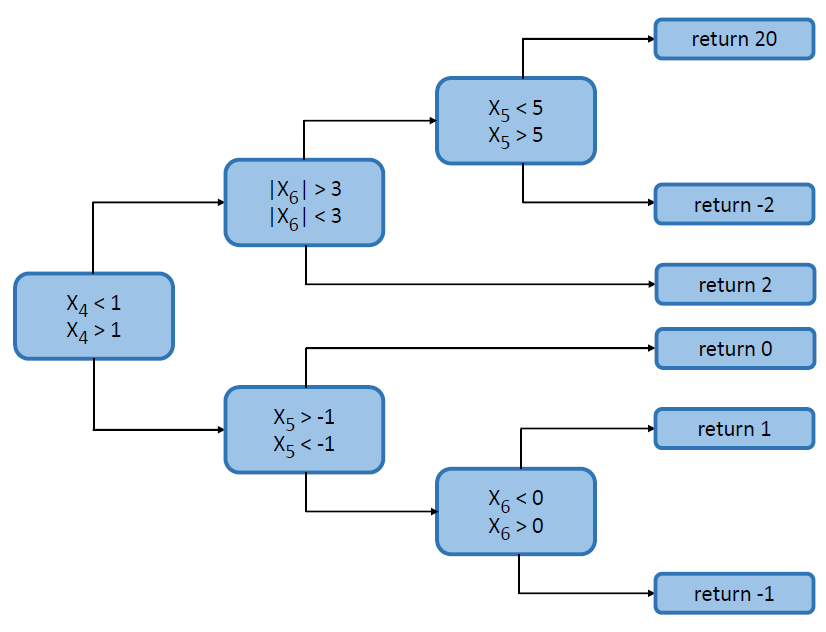
\includegraphics[width=0.5\textwidth]{tree_structure.png}
    \caption{Tree-like structure \(tree(x_{4},x_{5},x_{6})\) of the fixed effects part in Equation \refeq{eq:simstudy2}.}
    \label{fig:tree}
\end{figure}

The random effects are drawn from a normal distribution for two distinct scenarios:
\begin{itemize}
    \item \(Random \quad intercept \quad only: \sum_{q=0}^{Q} z_{qij}^T b_{qi} = b_{0i} \sim \mathcal{N}(0, \sigma^2_1)\), where \(\sigma^2_1\) is a design parameter which gives the possibility to change the variability of the effects in the different simulations.
    Indeed, within each scenario, two specifications (low and high) for the parameter \(\sigma^2_1\) are considered in order to account for different levels of magnitude of the between-group variability;
    \item \(Random \quad intercept \quad and \quad slope: \sum_{q=0}^{Q} z_{qij}^T b_{qi} = b_{0i} + x_{1ij}^T b_{1i}\), where \(x_{1ij}\) is the first fixed effects covariate and the random coefficient is \(\bm{b}_i \sim \mathcal{N}_2(0, \Sigma)\), with \(\Sigma=diag(\sigma^2_1;\sigma^2_2)\).
    It is important to note that the random effects \(b_{0i}\) and \(b_{1i}\) are treated as independent for any given value of \(i\), and as in the previous scenario \(\sigma^2_1\) and \(\sigma^2_2\) serves as parameters that regulates the random effects variance.
    In this setting, the covariate \(x_1\) is not assumed to have a fixed effect that applies uniformly across all observations. Instead, its impact is considered group-specific, meaning that \(x_1\) is assumed to have different effects across observations belonging to distinct groups.
\end{itemize}

In particular, a two-level data structure of \(I = 10\) groups with \(n_{i} = 100\) observations each is simulated, for a total number of units equal to 1000.
Note that for simplicity, an equal number of observations for each group is taken to ensure a balanced dataset. However, the model is, of course, capable of handling datasets with varying group sizes.

In addition to this simulation design approach, a more linear DGP is implemented in order to observe how OMERF method performs in a simpler context. In this case the first three covariates generated before are combined as follows:
\begin{equation}
    \label{eq:simstudy3}
    \begin{aligned}
        f(x_{1}, \dots,x_{3}) = 3+7x_{1}-5x_{2}+x_{2}x_{3}.
    \end{aligned}
\end{equation}
Only the case of a single, normally distributed random intercept is considered: \(b_{0i} \sim \mathcal{N}(0, \sigma^2_1)\).

All the design parameters listed before are chosen in order to obtain balanced simulated datasets regarding the classes of the ordinal response.
Moreover, several combinations of parameters are tested to observe how the model reacts in the case of a more polynomial or more tree-like response and with the variance related to random effects being higher or lower.
Thus, a total of 10 DGPs summarised in Table \ref{table:DGPs} are obtained. The main objective of the designed DGPs is to show how our algorithm is able to capture the variability of the groups and the nonlinear relationships of the data structure.
With these DGPs the OMERF's performance is evaluated in comparison to other three models: 
\begin{itemize}
    \item CLM and CLMM, from the \(ordinal\) R package \cite{ordinal}, which are expected to perform well in a linear context but are not able to model more complex structures, and in the case of CLM not even to grasp the hierarchical structure of data;
    \item Ordinal random forest, from the \(ordinalForest\) R package \cite{hornung2020ordinal}, which, as typical of ensemble tree-based models, is able to capture nonlinear relationships, but can not catch the nested structure.
\end{itemize}
These methods are chosen in order to, at least to some extent, include a range of both cumulative link and tree-based models.

\begin{table}[H]
    \centering 
    \begin{tabular}{|p{4em} | c | c | c | c | c |}
    \hline
    \rowcolor{bluePoli!40}
    & \textbf{\(f(\bm{x}_{ij})\)} & \textbf{\(\alpha\)} & \textbf{\(\beta\)} & \textbf{\(\sigma^2_1\)} & \textbf{\(\sigma^2_2\)} \T\B \\
    \hline \hline
    \textbf{DGP 1} & \(\alpha(3+7x_{1}^2-5x_{2}+x_{2}x_{3}^2) + \beta tree(x_{4},x_{5},x_{6})\) & 0.3 & 0.7 & 1 & - \T\B \\
    \textbf{DGP 2} & \(\alpha(3+7x_{1}^2-5x_{2}+x_{2}x_{3}^2) + \beta tree(x_{4},x_{5},x_{6})\) & 0.7 & 0.3 & 1 & - \T\B \\
    \textbf{DGP 3} & \(\alpha(3+7x_{1}^2-5x_{2}+x_{2}x_{3}^2) + \beta tree(x_{4},x_{5},x_{6})\) & 0.3 & 0.7 & 5 & - \T\B \\
    \textbf{DGP 4} & \(\alpha(3+7x_{1}^2-5x_{2}+x_{2}x_{3}^2) + \beta tree(x_{4},x_{5},x_{6})\) & 0.7 & 0.3 & 5 & - \T\B \\
    \textbf{DGP 5} & \(\alpha(3+7x_{1}^2-5x_{2}+x_{2}x_{3}^2) + \beta tree(x_{4},x_{5},x_{6})\) & 0.3 & 0.7 & 0.3 & 0.5 \T\B \\
    \textbf{DGP 6} & \(\alpha(3+7x_{1}^2-5x_{2}+x_{2}x_{3}^2) + \beta tree(x_{4},x_{5},x_{6})\) & 0.7 & 0.3 & 0.3 & 0.5 \T\B \\
    \textbf{DGP 7} & \(\alpha(3+7x_{1}^2-5x_{2}+x_{2}x_{3}^2) + \beta tree(x_{4},x_{5},x_{6})\) & 0.3 & 0.7 & 1 & 1 \T\B \\
    \textbf{DGP 8} & \(\alpha(3+7x_{1}^2-5x_{2}+x_{2}x_{3}^2) + \beta tree(x_{4},x_{5},x_{6})\) & 0.7 & 0.3 & 1 & 1 \T\B \\
    \textbf{DGP 9} & \(3+7x_{1}-5x_{2}+x_{2}x_{3}\) & - & - & 1 & - \T\B \\
    \textbf{DGP 10} & \(3+7x_{1}-5x_{2}+x_{2}x_{3}\) & - & - & 5 & - \B \\
    \hline
    \end{tabular}
    \\[10pt]
    \caption{Simulation parameters of both fixed and random effects parts for 10 different DGPs.}
    \label{table:DGPs}
\end{table}

\subsection{Simulation results}
\label{sec:simres}
For each of the ten DGPs described in Table \ref{table:DGPs} we simulate the dataset 100 times with 1000 observations each. In order to evaluate the predictive performances of the four compared models, each dataset is randomly split into training and test sets, with a ratio of 80\% for training and 20\% for testing.
To evaluate the quality of the predictions the five performance measures presented in Section \ref{sec:gof} are computed. Simulation results, consisting of mean and variance of each set of simulations for each index,  are reported in Tables \ref{table:res_int}, \ref{table:res_slope} and \ref{table:res_lin}.

From the findings reported in these tables, it can be inferred that generally, all performance measures in each simulation are consistent in the results. In particular, the performance of the created OMERF method is always good, and, even when not the best, remains mostly comparable to that of the top-performing model.

Note that the difference in effectiveness between tree-based methods (ordianl forest and OMERF) and linear models (CLM and CLMM) is especially significant when the DGP has a more tree-like structure (e.g. DGPs 1,3 in Table \ref{table:res_int}).
On the other hand, in cases where the DGP is based on a more polynomial structure (e.g. GDPs 2,4 in Table \ref{table:res_int}), the ordinal random forest and OMERF models still better capture the complexity of the problem, but the difference with the basic linear models is more negligible.
Indeed, the OMERF method reaches the best performance in DGP 2 (with \(Accuracy\) = 0.8039, \(MSE\) = 0.2646, \(ARI\) = 0.5324, \(Cohen's \, k\) = 0.5092, \(Cardoso \, idx\) = 0.2918, \(Ballante \, idx\) = 0.0960),
but has the largest difference in performance compared to the linear models in DGP 1, with an accuracy 0.0784 higher than CLM and 0.08 higher than CLMM.

Even with the introduction of a random slope (namely in the cases reported in Table \ref{table:res_slope}), the models' performance remains consistent with those analysed so far.
Moreover, in all the simulations there appear to be no major differences between the cases with small or large variability fixed effects.

On the contary, in DGPs 9 and 10 in Table \ref{table:res_lin}, which are specifically constructed with linear relationships, it is evident that CLM and CLMM tend to perform better with respect to the other models.
This result confirm that tree-based methods better capture nonlinear dependencies, but when there are linear data structures, simpler models are preferable, additionally yielding results that are usually more easily interpretable.

As for the variances in the estimations, all models estimates present small variability. Indeed, even OMERF is able to provide stable estimates, probably due to the iterative nature of the algorithm, which stabilizes the results.

Finally, since OMERF alternates between a random forest and a CLMM model, it takes the advantages of both methods.
Indeed, reporting in Figures \ref{fig:ranefDGP1} and \ref{fig:fix_cov_DGP1} the results in one of the runs of DGP 1 as a reference, it is evident how it succesfully manages to capture both the nested structure of the 10 random groups thanks to the CLMM, and the nonlinear relationships between the target value and the covariates, thanks to the RF.

\begin{figure}[H]
    \centering
    \subfloat[Original random coefficients taken from the normal distribution \(\sim \mathcal{N}(0, 1)\), as described in the simulation design in Section \ref{sec:simdesign}.\label{fig:original_re}]{
        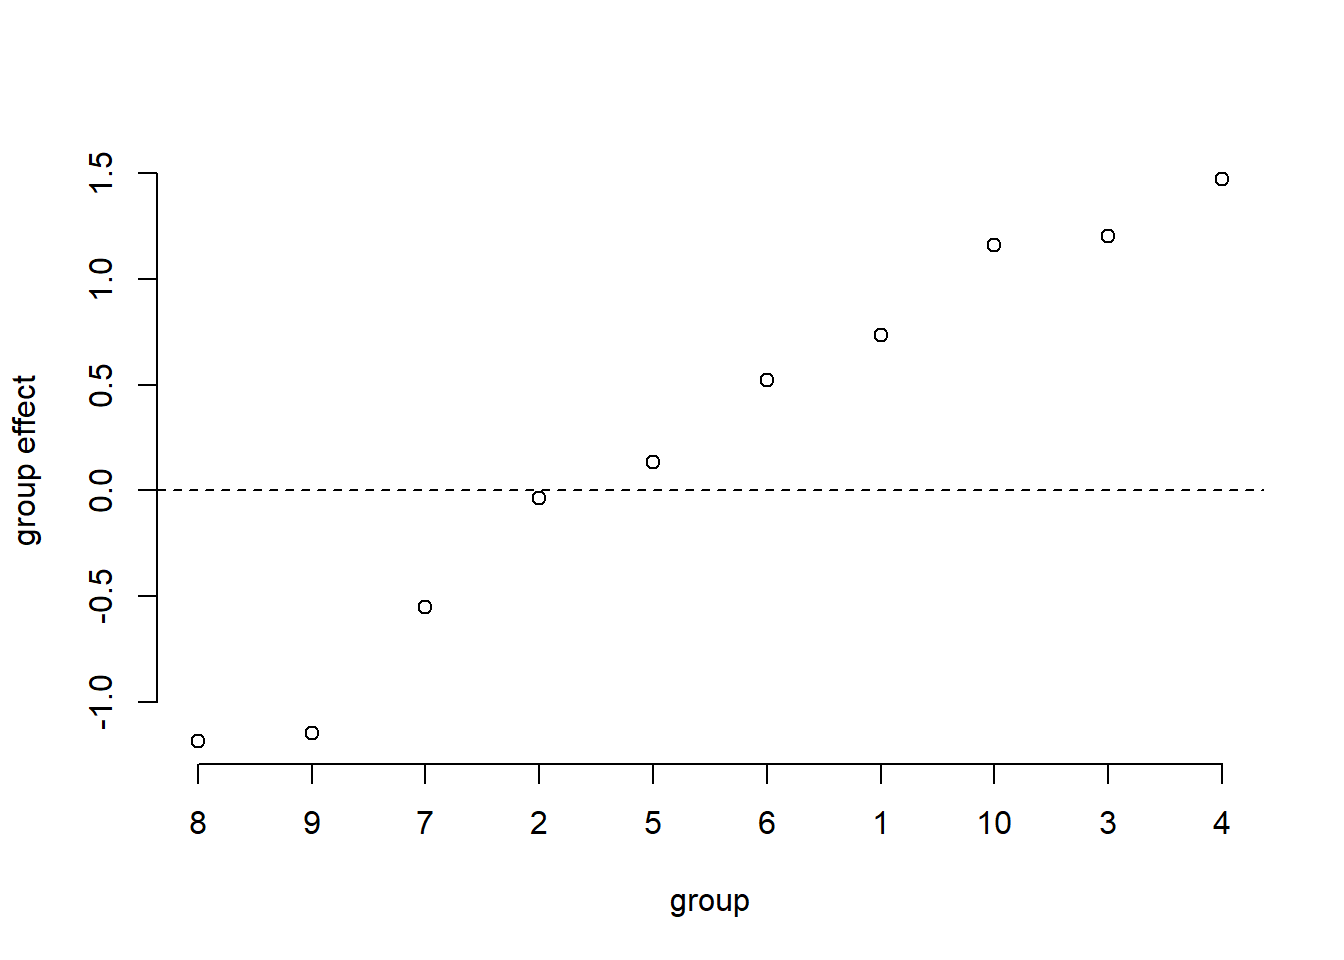
\includegraphics[scale=0.4]{Images/ranef1.png}
    }
    \quad
    \subfloat[Random intercepts with their confidence intervals, relative to the 10 simulated groups estimated by the OMERF method.\label{fig:estim_re}]{
        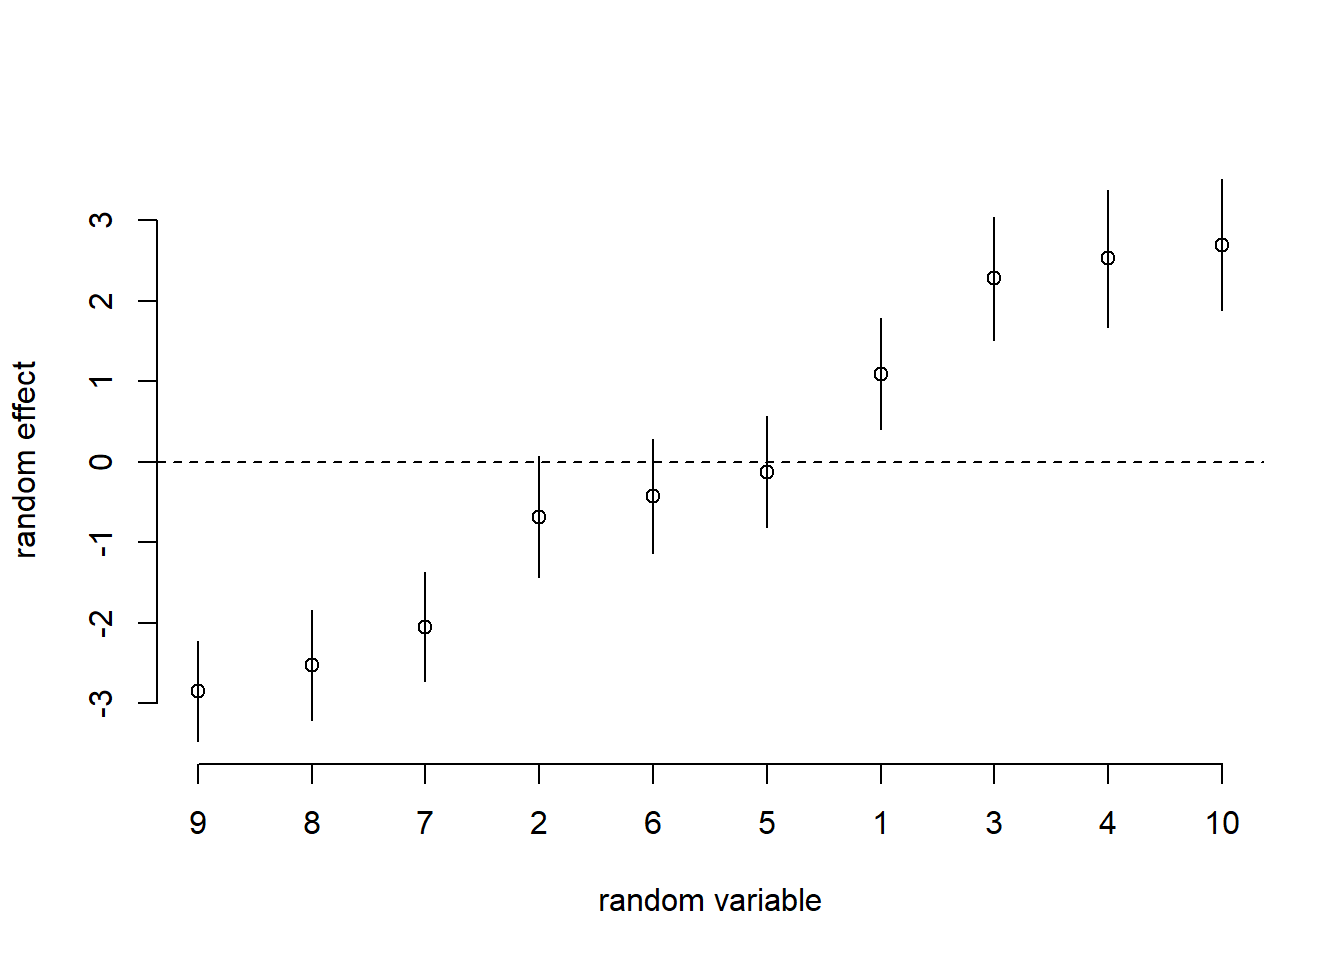
\includegraphics[scale=0.4]{Images/ranef2.png}
    }
    \caption[]{Random effects in one of the runs of DGP 1, listed in Table \ref{table:DGPs}.}
    \label{fig:ranefDGP1}
\end{figure}


\begin{figure}[H]
    \centering
    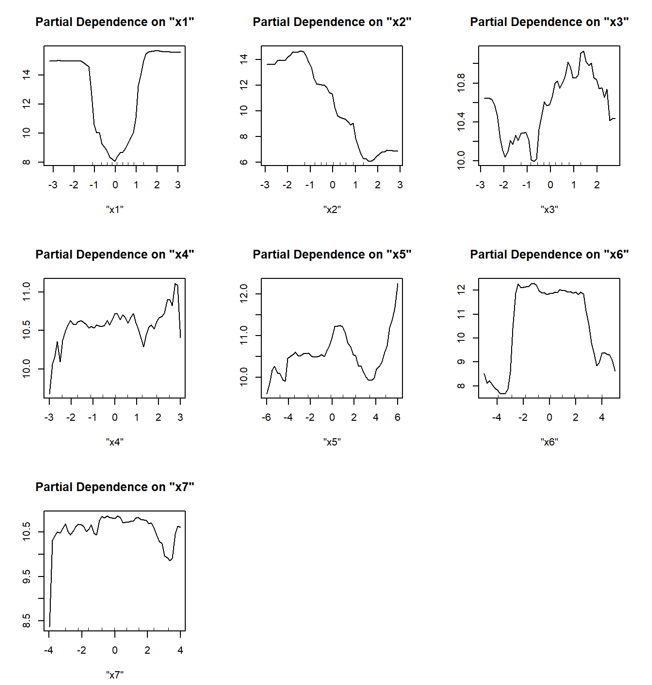
\includegraphics[width=0.8\textwidth]{fix_cov_sim.png}
    \caption{Partial plots of the random forest target value in the OMERF method with respect to the seven covariates of DGP 1, described in Table \ref{table:DGPs}. The \(y\)-axis reports the increment/decrement of the target value, given the covariate on the \(x\)-axis.}
    \label{fig:fix_cov_DGP1}
\end{figure}

Figure \ref{fig:ranefDGP1} recreates the differences in the hierarchical level (Figure \ref{fig:estim_re}) comapred to the original random coefficients taken from the normal distribution (Figure \ref{fig:original_re}).
Figure \ref{fig:fix_cov_DGP1} shows, on the other hand, the association of covariates and response, giving an insight into the underlying latent process behind the ordinal model. It can be observed that the algorithm captures the quadratic and inverse linear trend in the variables \(x_1\) and \(x_2\) respectively.

In conclusion, in a nonlinear setting the proposed method performs better with respect to CLM and CLMM, and comparably to ordinal random forest; having the advantage of increasing the knowledge about the multilevel nature of data.

\begin{table}[H]
    \centering 
    \begin{tabular}{|p{4em} c c c c c c c |}
    \hline
    \rowcolor{bluePoli!40}
    & \textbf{Model} & \textbf{Acc} & \textbf{MSE} & \textbf{ARI} & \textbf{Cohen's k} & \textbf{Cardoso} & \textbf{Ballante} \T\B \\
    \hline \hline
    \textbf{DGP 1} & clm & 0.5729 & 0.7074 & 0.1228 & 0.1650 &  0.5498 & 0.2731 \T\B \\
    \textbf{} &  & (0.0019) & (0.0109) & (0.0018) & (0.0032) & (0.0022) & (0.0013) \T\B \\
    \textbf{DGP 1} & clmm & 0.5713 & 0.7127 & 0.1176 & 0.1535 &  0.5503 & 0.2742 \T\B \\
    \textbf{} &  & (0.0018) & (0.0103) & (0.0017) & (0.0031) & (0.0021) & (0.0014) \T\B \\
    \textbf{DGP 1} & ordforest & 0.6491 & 0.5076 & 0.2588 & 0.3346 & 0.4619 & 0.1991 \T\B \\
    \textbf{} &  & (0.0009) & (0.0046) & (0.0024) & (0.0039) & (0.0013) & (0.0007) \T\B \\
    \textbf{DGP 1} & omerf & $\textcolor{bluePoli}{0.6564}$ & $\textcolor{bluePoli}{0.4532}$ & $\textcolor{bluePoli}{0.2958}$ & $\textcolor{bluePoli}{0.3975}$ & $\textcolor{bluePoli}{0.4617}$ & $\textcolor{bluePoli}{0.1981}$ \T\B \\
    \textbf{} &  & (0.0012) & (0.0036) & (0.0023) & (0.0028) & (0.0015) & (0.0007) \T\B \\
    \hline
    \textbf{DGP 2} & clm & 0.7496 & 0.5047 & 0.1923 & 0.2042 & 0.3811 & 0.1704 \T\B \\
    \textbf{} &  & (0.0008) & (0.0067) & (0.0035) & (0.0036) & (0.0016) & (0.0032) \T\B \\
    \textbf{DGP 2} & clmm & 0.7512 & 0.5061 & 0.1812 & 0.1962 & 0.3791 & 0.1806 \T\B \\
    \textbf{} &  & (0.0008) & (0.0063) & (0.0033) & (0.0035) & (0.0015) & (0.0040) \T\B \\
    \textbf{DGP 2} & ordforest & 0.8025 & 0.3148 & 0.3997 & 0.3954 & 0.2909 & $\textcolor{bluePoli}{0.0843}$ \T\B \\
    \textbf{} &  & (0.0006) & (0.0026) & (0.0042) & (0.0047) & (0.0011) & (0.0003) \T\B \\
    \textbf{DGP 2} & omerf & $\textcolor{bluePoli}{0.8090}$ & $\textcolor{bluePoli}{0.2572}$ & $\textcolor{bluePoli}{0.5331}$ & $\textcolor{bluePoli}{0.5086}$ & $\textcolor{bluePoli}{0.2835}$ & 0.0908 \T\B \\
    \textbf{} &  & (0.0008) & (0.0023) & (0.0039) & (0.0039) & (0.0016) & (0.0004) \T\B \\
    \hline
    \textbf{DGP 3} & clm & 0.6238 & 0.6589 & 0.2182 & 0.2943 &  0.5081 & 0.2314 \T\B \\
    \textbf{} &  & (0.0031) & (0.0197) & (0.0043) & (0.0054) & (0.0041) & (0.0025) \T\B \\
    \textbf{DGP 3} & clmm & 0.6236 & 0.6646 & 0.2156 & 0.2893 &  0.5082 & 0.2330 \T\B \\
    \textbf{} &  & (0.0031) & (0.0202) & (0.0044) & (0.0059) & (0.0041) & (0.0025) \T\B \\
    \textbf{DGP 3} & ordforest & 0.6705 & 0.5371 & 0.2853 & 0.3576 & 0.4490 & 0.1829 \T\B \\
    \textbf{} &  & (0.0016) & (0.0079) & (0.0038) & (0.0082) & (0.0022) & (0.0010) \T\B \\
    \textbf{DGP 3} & omerf & $\textcolor{bluePoli}{0.6741}$ & $\textcolor{bluePoli}{0.4591}$ & $\textcolor{bluePoli}{0.3340}$ & $\textcolor{bluePoli}{0.4222}$ & $\textcolor{bluePoli}{0.4471}$ & $\textcolor{bluePoli}{0.1785}$ \T\B \\
    \textbf{} &  & (0.0016) & (0.0049) & (0.0028) & (0.0037) & (0.0019) & (0.0008) \T\B \\
    \hline
    \textbf{DGP 4} & clm & 0.7532 & 0.5372 & 0.2389 & 0.2725 & 0.3843 & 0.2100 \T\B \\
    \textbf{} &  & (0.0015) & (0.0143) & (0.0036) & (0.0043) & (0.0031) & (0.0069) \T\B \\
    \textbf{DGP 4} & clmm & 0.7536 & 0.5377 & 0.2327 & 0.2659 & 0.3839 & 0.2118 \T\B \\
    \textbf{} &  & (0.0015) & (0.0138) & (0.0036) & (0.0047) & (0.0030) & (0.0071) \T\B \\
    \textbf{DGP 4} & ordforest & 0.7953 & 0.3708 & 0.3583 & 0.3722 & 0.3102 & 0.0998 \T\B \\
    \textbf{} &  & (0.0009) & (0.0059) & (0.0075) & (0.0080) & (0.0019) & (0.0010) \T\B \\
    \textbf{DGP 4} & omerf & $\textcolor{bluePoli}{0.8057}$ & $\textcolor{bluePoli}{0.2884}$ & $\textcolor{bluePoli}{0.5115}$ & $\textcolor{bluePoli}{0.5046}$ & $\textcolor{bluePoli}{0.2933}$ & $\textcolor{bluePoli}{0.0886}$ \T\B \\
    \textbf{} &  & (0.0012) & (0.0045) & (0.0047) & (0.0041) & (0.0024) & (0.0005) \B \\
    \hline
    \end{tabular}
    \\[10pt]
    \caption{Mean prediction performances (and their variances) of the four methods across 100 runs of the DGPs 1-4 of the ten simulation cases listed in Table \ref{table:DGPs}.}
    \label{table:res_int}
\end{table}

\begin{table}[H]
    \centering 
    \begin{tabular}{|p{4em} c c c c c c c |}
    \hline
    \rowcolor{bluePoli!40}
    & \textbf{Model} & \textbf{Acc} & \textbf{MSE} & \textbf{ARI} & \textbf{Cohen's k} & \textbf{Cardoso} & \textbf{Ballante} \T\B \\
    \hline \hline
    \textbf{DGP 5} & clm & 0.5598 & 0.7261 & 0.0970 & 0.1288 & 0.5604 & 0.2819 \T\B \\
    \textbf{} &  & (0.0009) & (0.0045) & (0.0012)  & (0.0026)  & (0.0008)  & (0.0006) \T\B \\
    \textbf{DGP 5} & clmm & 0.5586 & 0.7315 & 0.0940 & 0.1206 & 0.5611 & 0.2851 \T\B \\
    \textbf{} &  & (0.0009) & (0.0048) & (0.0014)  & (0.0029)  & (0.0009)  & (0.0009) \T\B \\
    \textbf{DGP 5} & ordforest & $\textcolor{bluePoli}{0.6409}$ & 0.5002 & 0.2541 & 0.3283 & $\textcolor{bluePoli}{0.4659}$ & $\textcolor{bluePoli}{0.2038}$ \T\B \\
    \textbf{} &  & (0.0009) & (0.0033) & (0.0025)  & (0.0033)  & (0.0013)  & (0.0005) \T\B \\
    \textbf{DGP 5} & omerf & 0.6339 & $\textcolor{bluePoli}{0.4948}$ & $\textcolor{bluePoli}{0.2636}$ & $\textcolor{bluePoli}{0.3623}$ & 0.4872 & 0.2170 \T\B \\
    \textbf{} &  & (0.0012) & (0.0041) & (0.0028)  & (0.0033)  & (0.0014)  & (0.0007) \T\B \\
    \hline
    \textbf{DGP 6} & clm & 0.7489 & 0.4900 & 0.1803 & 0.1854 & 0.3786 & 0.1653 \T\B \\
    \textbf{} &  & (0.0005) & (0.0036) & (0.0038)  & (0.0039)  & (0.0008)  & (0.0036) \T\B \\
    \textbf{DGP 6} & clmm & 0.7503 & 0.4927 & 0.1699 & 0.1812 & 0.3776 & 0.1771 \T\B \\
    \textbf{} &  & (0.0005) & (0.0041) & (0.0038)  & (0.0038)  & (0.0008)  & (0.0040) \T\B \\
    \textbf{DGP 6} & ordforest & 0.8063 & 0.2987 & 0.4187 & 0.4089 & $\textcolor{bluePoli}{0.2834}$ & $\textcolor{bluePoli}{0.0824}$ \T\B \\
    \textbf{} &  & (0.0004) & (0.0023) & (0.0040)  & (0.0049)  & (0.0008)  & (0.0003) \T\B \\
    \textbf{DGP 6} & omerf & $\textcolor{bluePoli}{0.8100}$ & $\textcolor{bluePoli}{0.2579}$ & $\textcolor{bluePoli}{0.5391}$ & $\textcolor{bluePoli}{0.5109}$ & 0.2837 & 0.0909 \T\B \\
    \textbf{} &  & (0.0007) & (0.0021) & (0.0042)  & (0.0042)  & (0.0013)  & (0.0005) \T\B \\
    \hline
    \textbf{DGP 7} & clm & 0.5696 & 0.7339 & 0.1205 & 0.1691 & 0.5571 & 0.2791 \T\B \\
    \textbf{} &  & (0.0015) & (0.0013) & (0.0020)  & (0.0039)  & (0.0019)  & (0.0020) \T\B \\
    \textbf{DGP 7} & clmm & 0.5643 & 0.7491 & 0.1119 & 0.1571 & 0.5630 & 0.2848 \T\B \\
    \textbf{} &  & (0.0018) & (0.0013) & (0.0021)  & (0.0045)  & (0.0021)  & (0.0022) \T\B \\
    \textbf{DGP 7} & ordforest & $\textcolor{bluePoli}{0.6414}$ & 0.5334 & 0.2554 & 0.3254 & $\textcolor{bluePoli}{0.4719}$ & $\textcolor{bluePoli}{0.2074}$ \T\B \\
    \textbf{} &  & (0.0011) & (0.0047) & (0.0022)  & (0.0031)  & (0.0015)  & (0.0008) \T\B \\
    \textbf{DGP 7} & omerf & 0.6335 & $\textcolor{bluePoli}{0.5130}$ & $\textcolor{bluePoli}{0.2695}$ & $\textcolor{bluePoli}{0.3581}$ & 0.4890 & 0.2172 \T\B \\
    \textbf{} &  & (0.0016) & (0.0066) & (0.0033)  & (0.0036)  & (0.0019)  & (0.0011) \T\B \\
    \hline
    \textbf{DGP 8} & clm & 0.7507 & 0.4943 & 0.2032 & 0.2139 & 0.3774 & 0.1729 \T\B \\
    \textbf{} &  & (0.0008) & (0.0073) & (0.0040)  & (0.0040)  & (0.0017)  & (0.0036) \T\B \\
    \textbf{DGP 8} & clmm & 0.7498 & 0.4985 & 0.1908 & 0.2029 & 0.3789 & 0.1809 \T\B \\
    \textbf{} &  & (0.0008) & (0.0069) & (0.0042)  & (0.0047)  & (0.0016)  & (0.0040) \T\B \\
    \textbf{DGP 8} & ordforest & 0.8011 & 0.3235  & 0.4025 & 0.3995 & $\textcolor{bluePoli}{0.2947}$ & $\textcolor{bluePoli}{0.0885}$ \T\B \\
    \textbf{} &  & (0.0005) & (0.0032) & (0.0047)  & (0.0041)  & (0.0011)  & (0.0003) \T\B \\
    \textbf{DGP 8} & omerf & $\textcolor{bluePoli}{0.8025}$ & $\textcolor{bluePoli}{0.2771}$ &  $\textcolor{bluePoli}{0.5182}$ & $\textcolor{bluePoli}{0.4964}$ & 0.2950 & 0.0961 \T\B \\
    \textbf{} &  & (0.0009) & (0.0037) & (0.0036)  & (0.0038)  & (0.0019)  & (0.0005) \B \\
    \hline
    \end{tabular}
    \\[10pt]
    \caption{Mean prediction performances (and their variances) of the four methods across 100 runs of the DGPs 5-8 of the ten simulation cases listed in Table \ref{table:DGPs}.}
    \label{table:res_slope}
\end{table}


\begin{table}[H]
    \centering 
    \begin{tabular}{|p{4em} c c c c c c c |}
    \hline
    \rowcolor{bluePoli!40}
    & \textbf{Model} & \textbf{Acc} & \textbf{MSE} & \textbf{ARI} & \textbf{Cohen's k} & \textbf{Cardoso} & \textbf{Ballante} \T\B \\
    \hline \hline
    \textbf{DGP 9} & clm & 0.8711 & 0.1610 & 0.7291 & 0.7761 & 0.1979 & 0.0419 \T\B \\
    \textbf{} &  & (0.0005) & (0.0016) & (0.0021)  & (0.0015)  & (0.0012)  & (0.0001) \T\B \\
    \textbf{DGP 9} & clmm & $\textcolor{bluePoli}{0.8716}$ & $\textcolor{bluePoli}{0.1609}$ & $\textcolor{bluePoli}{0.7297}$ & $\textcolor{bluePoli}{0.7769}$ & $\textcolor{bluePoli}{0.1977}$ & $\textcolor{bluePoli}{0.0417}$ \T\B \\
    \textbf{} &  & (0.0004) & (0.0014) & (0.0019)  & (0.0012)  & (0.0009)  & (0.0001) \T\B \\
    \textbf{DGP 9} & ordforest & 0.8544 & 0.2145 & 0.6858 & 0.7414 & 0.2262 & 0.0484 \T\B \\
    \textbf{} &  & (0.0004) & (0.0024) & (0.0022)  & (0.0013)  & (0.0012)  & (0.0002) \T\B \\
    \textbf{DGP 9} & omerf & 0.8374 & 0.2730 & 0.6477 & 0.7101 & 0.2533 & 0.0826 \T\B \\
    \textbf{} &  & (0.0004) & (0.0029) & (0.0025)  & (0.0012)  & (0.0012)  & (0.0002) \T\B \\
    \hline
    \textbf{DGP 10} & clm & $\textcolor{bluePoli}{0.8756}$ & $\textcolor{bluePoli}{0.1559}$ & $\textcolor{bluePoli}{0.7376}$ & $\textcolor{bluePoli}{0.7824}$ & $\textcolor{bluePoli}{0.1919}$ & 0.0386 \T\B \\
    \textbf{} &  & (0.0004) & (0.0012) & (0.0019)  & (0.0013)  & (0.0009)  & (9.1742e-05) \T\B \\
    \textbf{DGP 10} & clmm & 0.8755 & $\textcolor{bluePoli}{0.1559}$ & $\textcolor{bluePoli}{0.7376}$ & 0.7821 & 0.1920 & $\textcolor{bluePoli}{0.0385}$ \T\B \\
    \textbf{} &  & (0.0004) & (0.0011) & (0.0017)  & (0.0012)  & (0.0009)  & (9.0919e-05) \T\B \\
    \textbf{DGP 10} & ordforest & 0.8420 & 0.2610 & 0.6492 & 0.7154 & 0.2486 & 0.0523 \T\B \\
    \textbf{} &  & (0.0005) & (0.0031) & (0.0025)  & (0.0013)  & (0.0012)  & (0.0001) \T\B \\
    \textbf{DGP 10} & omerf & 0.8219 & 0.3328 & 0.6006 & 0.6784 & 0.2835 & 0.2142 \T\B \\
    \textbf{} &  & (0.0005) & (0.0055) & (0.0036)  & (0.0014)  & (0.0015)  & (0.0005) \B \\
    \hline
    \end{tabular}
    \\[10pt]
    \caption{Mean prediction performances (and their variances) of the four methods across 100 runs of the DGPs 9,10 of the ten simulation cases listed in Table \ref{table:DGPs}.}
    \label{table:res_lin}
\end{table}




\section{Case study}
\label{sec:case}
In this section a real life application of OMERF method is analysed, comparing its performance with that of the models already presented in Section \ref{sec:sim}.
The data used concern 427 students of a prestigious high school in Milan, containing  all the personal information stored in the school's electronic register.
The objective of this section is to explore and analyse potential approaches used to predict students' academic achievements and search the factors influencing these outcomes.
The final aim is to identify students who may be at risk of failure and generally to predict their academic progress.
Such insights enable the design and implementation of strategies to create tailored plans to enhance academic performance. Indeed, if it were possible to know promptly to which profile a student belongs, tutors and teachers could improve counselling actions and propose personalized learning.

In Section \ref{sec:dataset} and \ref{sec:exp_analisys} the dataset and its pre-processing are described and explored, while in Section \ref{sec:modres} the model results are presented.

\subsection{The dataset}
\label{sec:dataset}
The dataset concerns current and previous performance data of students enrolled in a high school in Milan in the academic years 2017/2018 and 2018/2019.
Students can be enrolled into 4 tracks: \(Liceo \, Classico \, Paritario\), \(Liceo \, Scienze \, Umane \, Paritario\), \(Liceo \, Scientifico \, Paritario\) and \(Liceo \, Internazionale \, per \, l'Intercultura\).

The infromation provided are mainly of two categories:
\begin{itemize}
    \item static or fixed information, i.e. information known before the beginning of the academic year or final information of it;
    \item periodic information, i.e. information deriving from the electronic register during each school week.
\end{itemize}
The aggregated data come from 9 different datasets, each one containing different information about all the students in the school in these two academic years:
\begin{itemize}
    \item \(dataset \, 1\): static information about each student and her personal and demographic characteristics;
    \item \(dataset \, 2\): static information about 27 classes in the whole school complex, such as the number of teachers and tenured teachers;
    \item \(dataset \, 3 \, \& \, 4\): weekly update regarding the days and the amount of hours of absence of each student;
    \item \(dataset \, 5\): weekly update regarding the number of notes of each student, which are classified as: merit notes, disciplinary notes and commitment notes;
    \item \(dataset \, 6\): weekly update regarding the number of delays of each student;
    \item \(dataset \, 7 \, \& \, 8\): weekly update regarding the students' test grades of each subject;
    \item \(dataset \, 9\): final grades of each student in each subject at the end of each period.
\end{itemize}

In particular, in our study we focus on student performance in mathematics, considering the following fixed covariates:
\begin{itemize}
    \item \(regular\): categorical variable indicating whether the student is age-matched (0), one or more years older than her peers (+1) or one or more years younger (-1);
    \item \(gender\): binary variable indicating student's gender (1=Male, 0=Female);
    \item \(nationality\): binary variable with value 1 if the student has Italian citizenship and 0 otherwise;
    \item \(PDB\): binary variable with value 1 if the student follows a personalized teaching plan ("Piano Didattico Personalizzato") and 0 otherwise;
    \item \(tenured \, teachers\): percentage of tenured teachers compared to the total number of teachers in the class;
    \item \(first \, term \, math\): mathematical grade of each student for the first half of the year;
    \item \(absence\): percentage of days of absence of each student in relation to the total number of school days, updated to the first half of the year;
    \item \(merit \, notes\): number of merit notes of each student, updated to the first half of the year;
    \item \(disciplinary \, notes\): categorical variable indicating the number of disciplinary notes of each student, updated to the first half of the year;
    \item \(commitment \, notes\): number of commitment notes of each student, updated to the first half of the year;
    \item \(delays\): number of delays of each student, updated to the first half of the year;
    \item \(variance\): variance of the mathematical grades taken up to the first half of the year, calculated in order to capture the fluctuations of each student's grade;
    \item \(previous \, math \, grade\): mathematical grade of each student for the previous academic year.
\end{itemize}
The types of variable and their specific domains are reported in Table \ref{table:fix_var}.

With regard to the random effects part, in our case study, students are naturally nested within classes but further levels of hierarchy are possible, such as the four different school types.

In the implemented model the ordinal response variable is the final mathematical grade of each student at the end of the academic year, which ranges from 4 to 10.
Indeed, the hypothesis is that considering a combination of background and performance indicators, updated up to the first half of the year, is enough to identify the students at risk and to draw the attention of tutors.
Moreover, in order to design an ordinal model that has fewer levels of the response variable than those of the final mathematical grade, we create a novel response variable, called \(risk\), which takes value 1 if the student's final grade in mathematics is equal to 4 or 5,
takes value 2 if it is equal to 6 or 7 and  takes value 3 if it is equal to 8, 9 or 10.

\begin{table}[H]
    \centering 
    \begin{tabular}{|p{10em}|c|c|}
    \hline
    \rowcolor{bluePoli!40}
    \textbf{Variable name} & \textbf{Type of variable} & \textbf{Domain} \T\B \\
    \hline \hline
    \(regular\) &  Factor &  \(\left\{-1,0,1\right\}\) \T\B \\
    \hline
    \(gender\) &  Factor &  \(\left\{0,1\right\}\) \T\B \\
    \hline
    \(nationality\) &  Factor &  \(\left\{0,1\right\}\) \T\B \\
    \hline
    \(PDB\) &  Factor &  \(\left\{0,1\right\}\) \T\B \\
    \hline
    \(tenured \, teachers\) &  Numeric &  \([0.72,1]\) \T\B \\
    \hline
    \(first \, term \, math\) &  Integer &  \(\left\{3,\dots,10\right\}\) \T\B \\
    \hline
    \(absence\) &  Numeric &  \([0,0.29]\) \T\B \\
    \hline
    \(merit \, notes\) &  Integer &  \(\left\{0,\dots,4\right\}\) \T\B \\
    \hline
    \(disciplinary \, notes\) &  Factor & \(\left\{0,1,2\right\}\) \T\B \\
    \hline
    \(commitment \, notes\) &  Integer &  \(\left\{0,\dots,11\right\}\) \T\B \\
    \hline
    \(delays\) &  Integer &  \(\left\{0,\dots,17\right\}\) \T\B \\
    \hline
    \(variance\) &  Numeric &  \([0,8.4]\) \T\B \\
    \hline
    \(previous \, math \, grade\) &  Integer &  \(\left\{2,\dots,10\right\}\) \B \\
    \hline
    \end{tabular}
    \\[10pt]
    \caption{Fixed covariates taken from the dataset analysed in Section \ref{sec:case}.}
    \label{table:fix_var}
\end{table}


\subsection{Exploratory data analysis}
\label{sec:exp_analisys}
From the demographic information, it can be noticed that there is a clear gender balance, with 209 females and 218 males. The majority of the students have Italian nationality, with only 10 foreign students coming from Chile, China, France, Japan, Peru, Russia, Spain and Switzerland.
There are 348 students of the appropriate age for their respective classes, 55 students who are one year younger than their peers, and 24 who are one year older. Among all the students, only 67 have a PDB (Personalized Development Plan).

In order to be able to take into account both performance data related to the previous and current academic year, we consider students from the second to the fifth class: there are 128 second-years, 125 third-years, 89 fourth-years and 85 final-years.
Only 68 students attend the \(Liceo \, Classico \, Paritario\), 105 students attend the \(Liceo \, Scienze \, Umane \, Paritario\), 105 students attend the \(Liceo \, Scientifico \, Paritario\) and finally, most of the students, i.e. 149, attends the \(Liceo \, Internazionale \, per \, l'Intercultura\).

In Figure \ref{fig:math} it is reported the students' final mathematical  grade distribution, while in Figures \ref{fig:box} and \ref{fig:ass} there is a comparison between the main covariates and the ordinal response.
From these images, it can be observed that certain covariates, such as gender, appear to have no association to the mathematical outcomes. In contrast, the results of students from different classes seem to vary.
From the distributions of the number of absences, notes, and delays, it can be noted that the majority of students have few of each of these, and there appears to be only a slight correlation with the final mathematical result.

\begin{figure}[H]
    \centering
    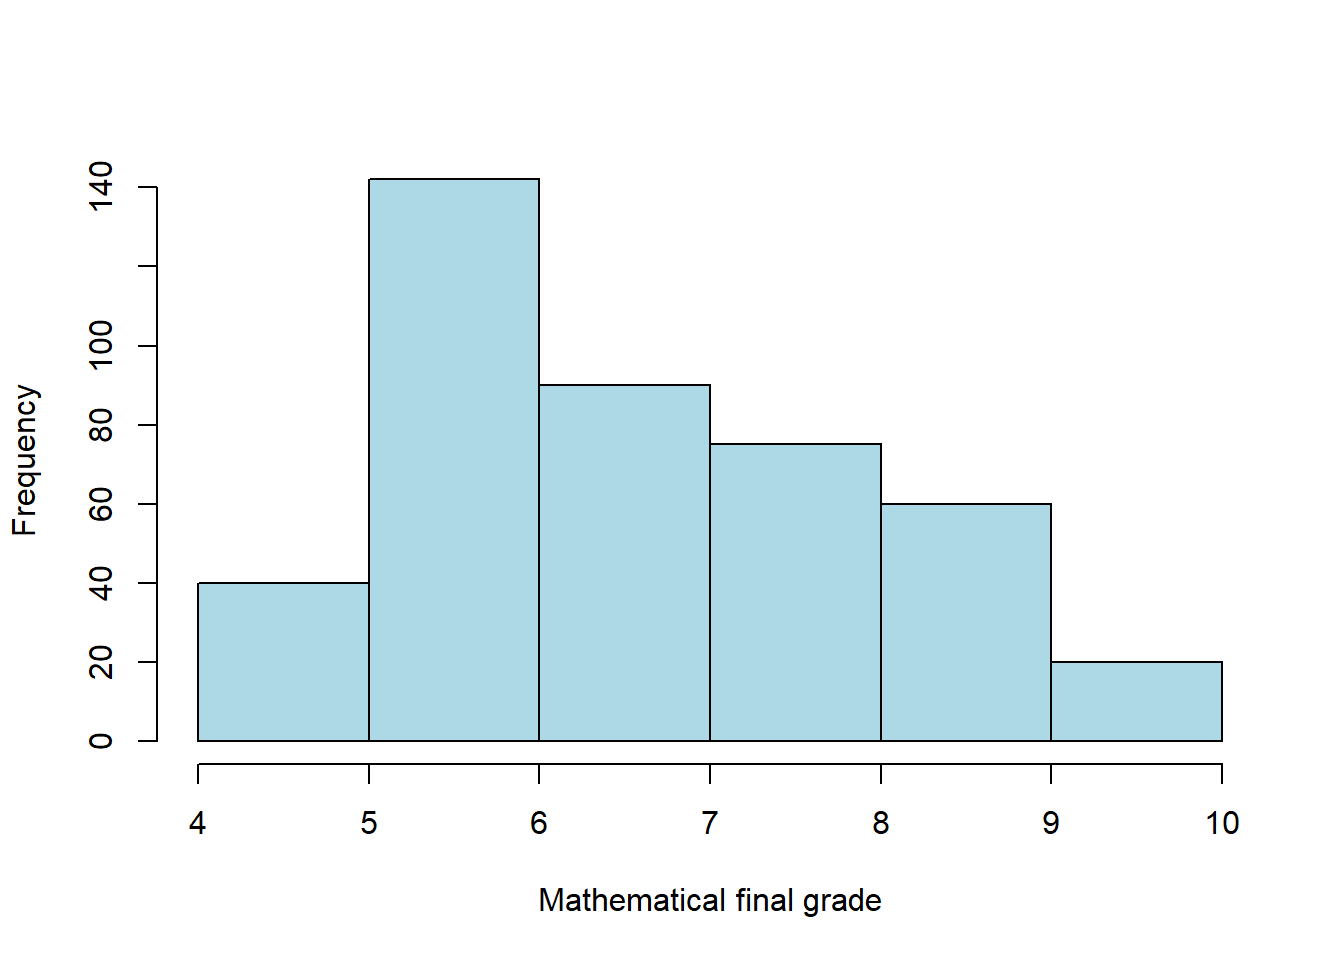
\includegraphics[width=0.30\textwidth]{math_final.png}
    \caption{Students' final mathematical grade distribution.}
    \label{fig:math}
\end{figure}

\begin{figure}[H]
    \centering
    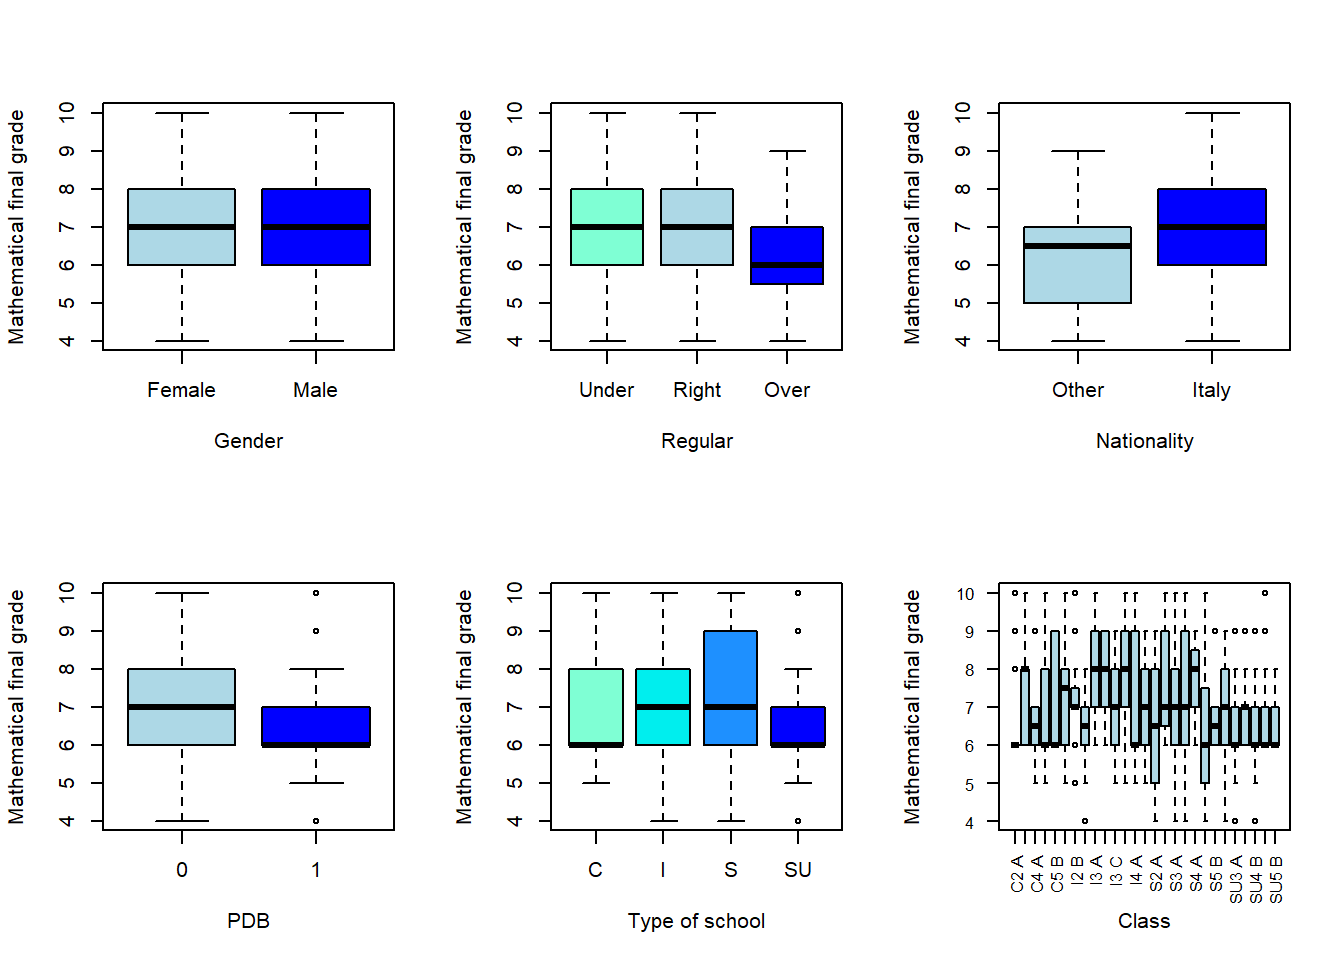
\includegraphics[width=0.75\textwidth]{boxplot_2.png}
    \caption{Comparison between \(gender, \, regular, \, nationality, \, PDB, \, type\,of\,school, \, class\) covariates and mathematical final evaluation.}
    \label{fig:box}
\end{figure}

\begin{figure}[H]
    \centering
    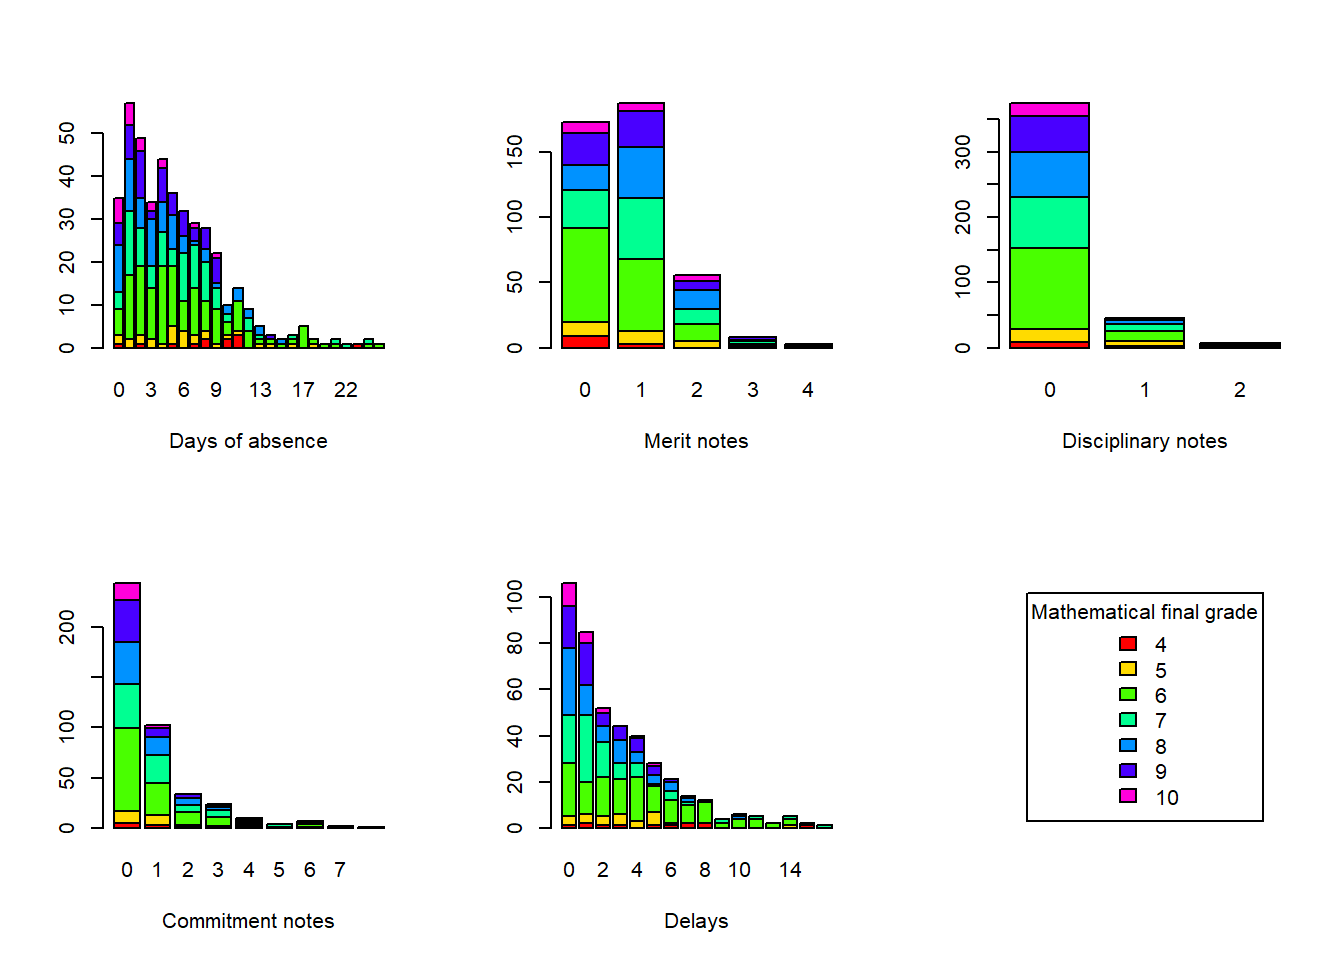
\includegraphics[width=0.8\textwidth]{assenze.png}
    \caption{Comparison between \(absence, \, merit\,notes, \, disciplinary\,notes, \, commitment\,notes, \, delays\) covariates and mathematical final evaluation.}
    \label{fig:ass}
\end{figure}







\subsection{Model results}
\label{sec:modres}
In the same way as in the simulation study, in order to evaluate the predictive performances of the four compared models, the dataset is randomly split into training and test sets, with a ratio of 80\% for training and 20\% for testing.

As mentioned in Section \ref{sec:dataset} two types of mixed-effects models are implemented: the first ones with ordinal response variable the student's final grade in mathematics, the others with ordinal response the created variable \(risk\).
For each collection of models three different set of covariates are tested:
\begin{itemize}
    \item all varaibles listed in Table \ref{table:fix_var}, excluding the ones related to the school performance in mathematics (i.e. \(first \, term \, math\), \(variance\), \(previous \, math \, grade\));
    \item all varaibles listed in Table \ref{table:fix_var}, excluding the ones related to the previous year school performance in mathematics (i.e. \(previous \, math \, grade\));
    \item all varaibles listed in Table \ref{table:fix_var}.
\end{itemize}
The choice of monitoring the differences among the three sets of covariates is done in order to observe the OMERF method's efficiency in various settings.
Indeed, the student's achievements in mathematics during the first half of the year and related to the previous year are expected to be highly linearly correlated with the model response.
The importance of this dependence with the target variable will greately influence the model estimates, and thus impact the model performances, probably favoring the simplest models, as emerged from the simulation study in Section \ref{sec:simres}.
For this reason, various combinations of variables are implemented with the aim of recording results even in a less strictly linear context and observing the behaviour of covariates that potentially have nonlinear trends.

In all these models a random intercept \(b_0\) for the student's class is included.

The prediction performances are reported in Tables \ref{table:res_math} and \ref{table:res_risk}.
From the results in Table \ref{table:res_math} it is clear that all the models exhibit poor predictive capabilities; this is probably due to the large number of levels of the considered response, which makes it difficult for models to distinguish between them.
In Table \ref{table:res_risk} in fact, having a three-level target variable, the performances are significantly better.
Moreover, it can be noticed that in the latter setting, in the first two cases implemented, the differences between all the models are subtler.
On the contrary, with the last set of covariates the rest of the models tend to overperform OMERF, sufficiently covering the level of complexity required by the problem. This phenomenon perfectly follows our previously stated hypothesis;
i.e. the information regarding the students' mathematical achievements has a linear relationship with the target values, and thus the existing models are best suited to this type of problem, reaching highest forecasting abilities when also the information concerning the 2017/2018 academic year is included.

Nevertheless, from OMERF's outputs can be retrieved meaningful information. Focusing on the second collection of models with \(risk\) response variable, all the three models highlight a similar hierarchical structure, as it is evident from the estimates of random intercepts shown in Figure \ref{fig:reff}.
Since the first model has less predictive power with respect to the other two, this reflectes in its lower ability to outline the nested structure; but it is in any case clear, even though less significant, the trend of random effects between classes.
Therefore, there is a visible difference in the performances of students belonging to different classes, as already noted in the exploratory analysis in Figure \ref{fig:box}. However, only a few classes have an intercepts significantly different from 0 (with 95\% confidence), deviating from the average.
In particular, there is not a recognisable pattern related to the age of the students in the classes or related to the different types of school. Instead, the class effect, net to the fixed effects contribution, might be due to having different teaching staff.

As the variance of the standard logistic distribution is \(\pi^2 / 3 \cong 3.29\), and the variance of the random effects in the three models are \(\sigma^2_{m4} = 0.5619,\quad \sigma^2_{m5} = 2.3345,\quad \sigma^2_{m6} = 1.8302\), the Intraclass Correlation Coefficients (ICCs) for the underlying linear
models can be estimated as:
\begin{gather*}
    \begin{aligned}
        ICC_4 = \frac{\sigma^2_{m4}}{\sigma^2_{m4}+\pi^2 / 3}= 0.1459, \quad ICC_5 = \frac{\sigma^2_{m5}}{\sigma^2_{m5}+\pi^2 / 3}= 0.4151, \quad ICC_6 = \frac{\sigma^2_{m6}}{\sigma^2_{m6}+\pi^2 / 3}= 0.3574.
    \end{aligned}
\end{gather*}
These values of ICC, measuring the unexplained variance in the response that can be atributed to the nested structure of students, together with the fact that some random intercepts are significantly different from zero (Figure \ref{fig:reff})
imply the existence of a substantial heterogeneity in the achievements among various classes. This highlight once again the importance of considering the hierarchical structure of these data.

\begin{figure}[H]
    \centering
    \subfloat[Model with all variables listed in Table \ref{table:fix_var}, excluding \(first \, term \, math\), \(variance\), \(previous \, math \, grade\).]{
        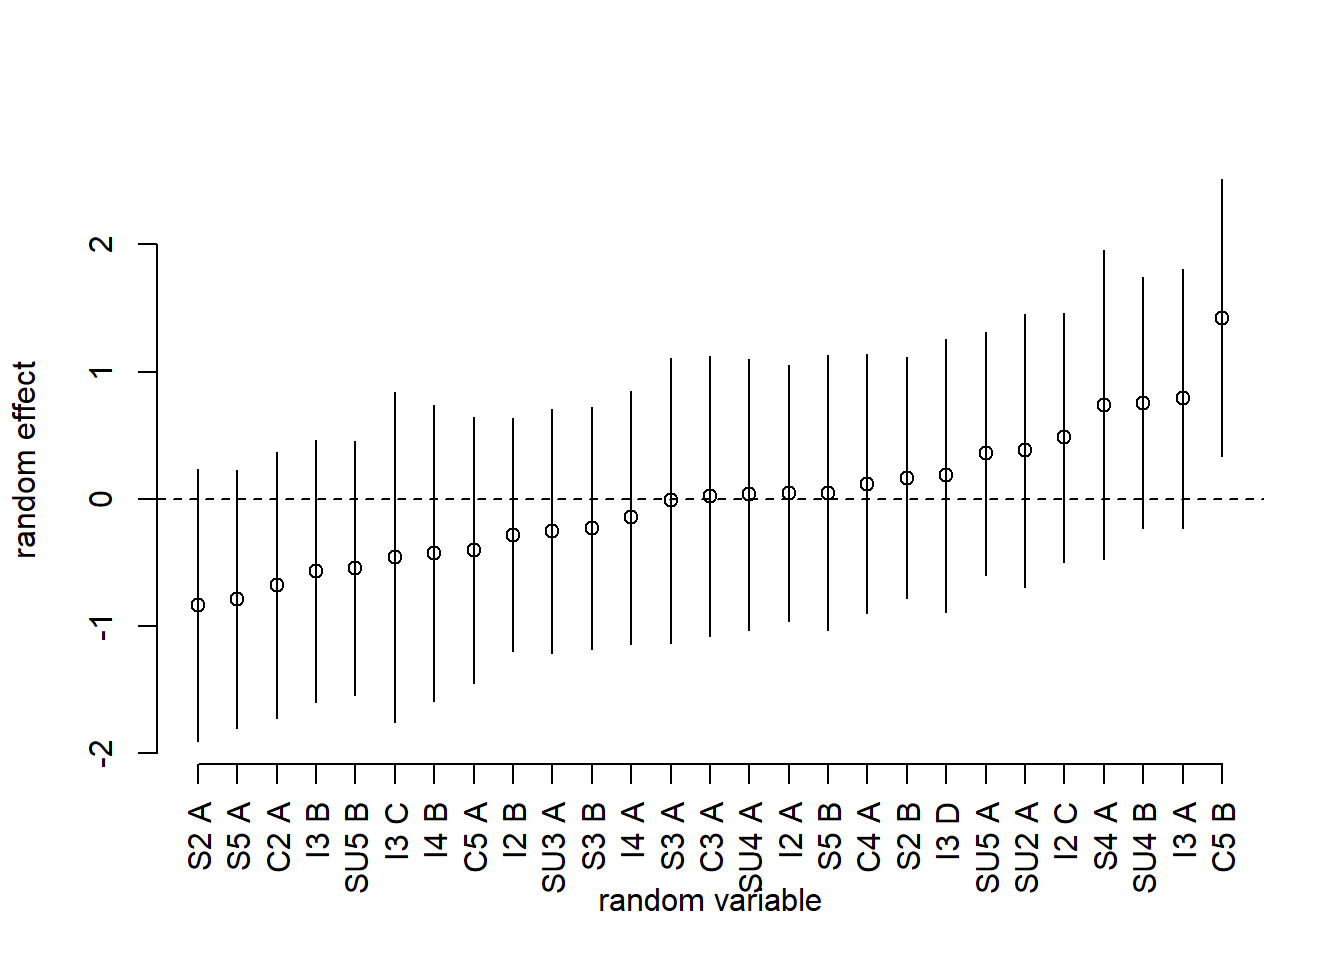
\includegraphics[scale=0.4]{Images/re0_3.png}
    }
    \quad
    \subfloat[Model with all variables listed in Table \ref{table:fix_var}, excluding \(previous \, math \, grade\).]{
        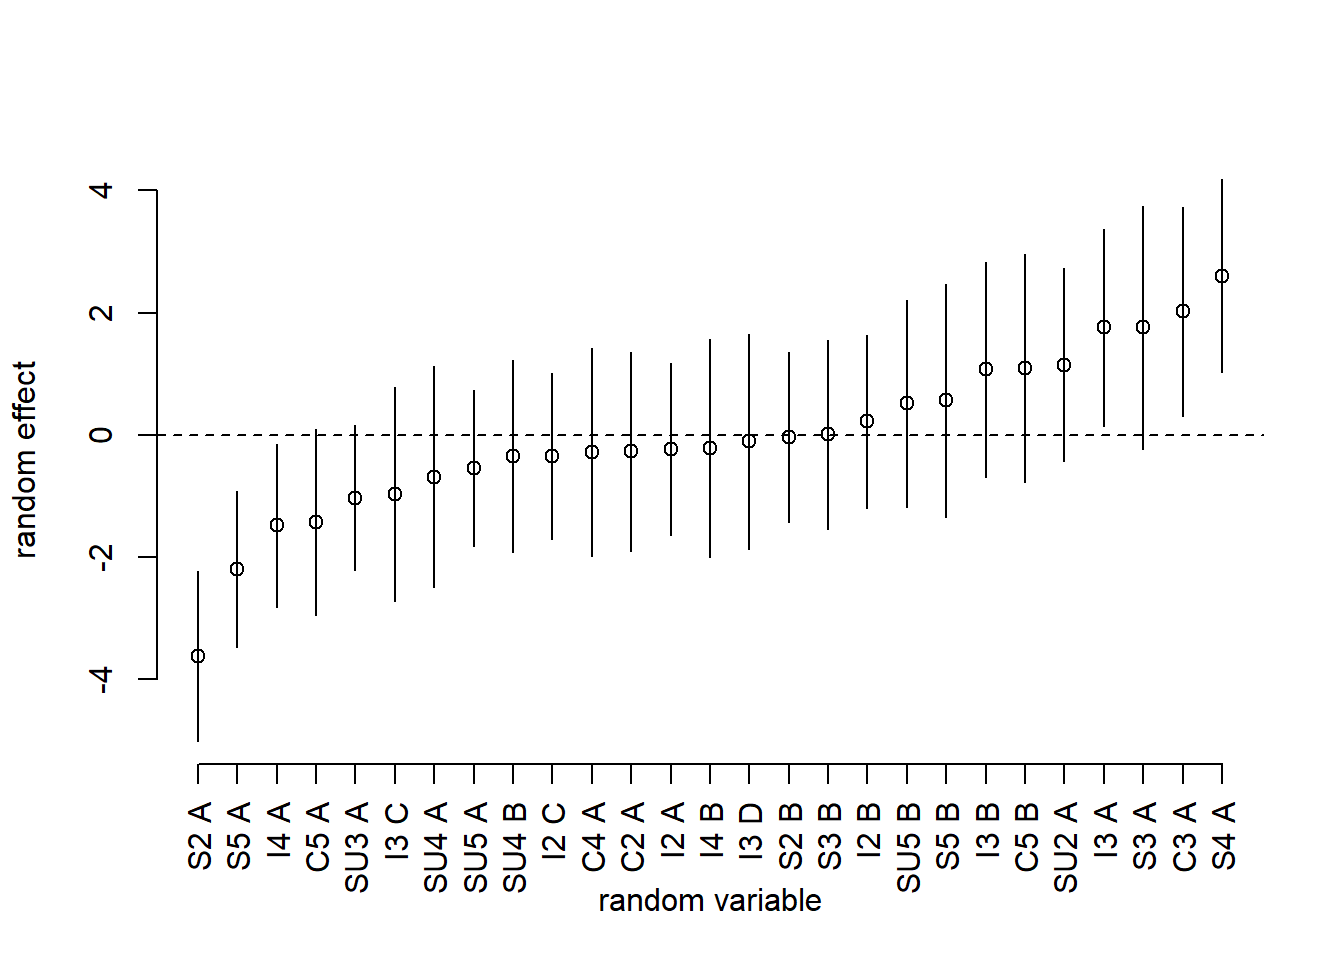
\includegraphics[scale=0.4]{Images/re1_3.png}
    }
    \quad
    \subfloat[Model with all variables listed in Table \ref{table:fix_var}.]{
        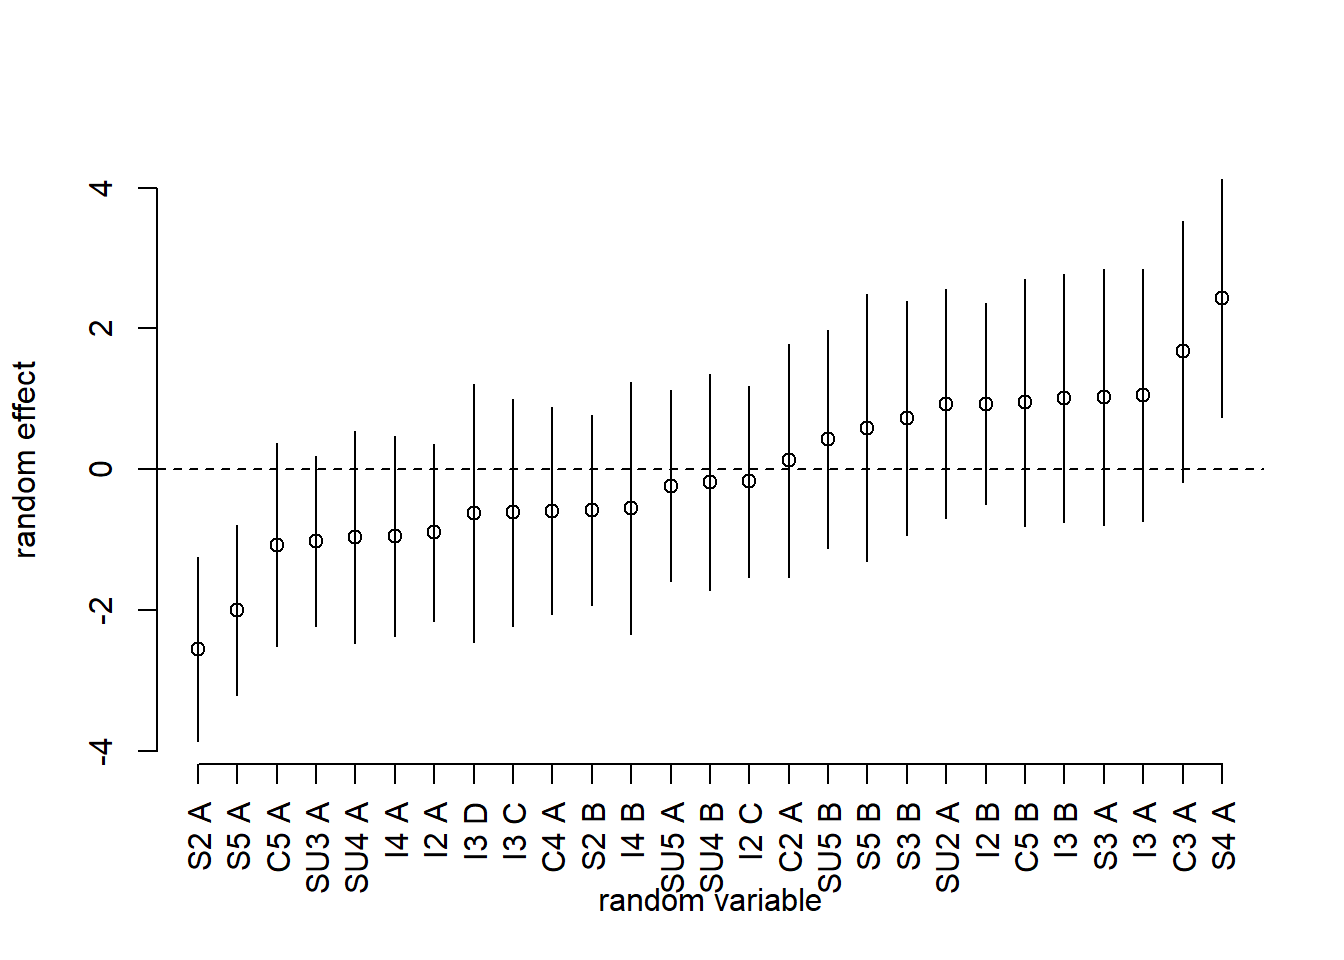
\includegraphics[scale=0.4]{Images/re2_3.png}
    }
    \caption[]{Random intercepts with their confidence intervals, relative to the 27 classes estimated by the OMERF model.}
    \label{fig:reff}
\end{figure}

Regarding the fixed effects, RF model in the OMERF algorithm measures the imporance of each covariate in explaining the response and the partial effect of each covariate.
Figure \ref{fig:varimp} shows dotcharts of the importance of the variables in the three models, as measured by two different indices.
The first index is derived from permuting out-of-bag data: for each tree, the prediction error (MSE for regression) on the out-of-bag portion of the data is recorded. Subsequently, the same process is repeated after permuting each predictor variable. The discrepancy between these two measures is then averaged across all trees comprising the random forest and normalized by the standard deviation of the differences.
The second index is the total decrease in node impurities resulting from splitting on the variable, averaged over all trees. In the context of regression, node impurity is quantified by the residual sum of squares.

As expected, when the covariates regarding mathematical performances are included in the models, they are of total importance, reducing the influence of others. In any case, the importance of the other covariates appears to be in line with what was evidenced by the boxplots in Figure \ref{fig:box}.
Specifically, by adding in the last two models the variables related to students' performance at school, the other covariates remain consistent, with \(absence\), \(delays\), \(PDB\) and \(tenuered \, teachers\) being generally the most important ones. This reflects the fact that even the first is a valid model despite having less predictive capabilities.

\begin{figure}[H]
    \centering
    \subfloat[Variable importance plot of the model with all variables listed in Table \ref{table:fix_var}, excluding \(first \, term \, math\), \(variance\), \(previous \, math \, grade\).]{
        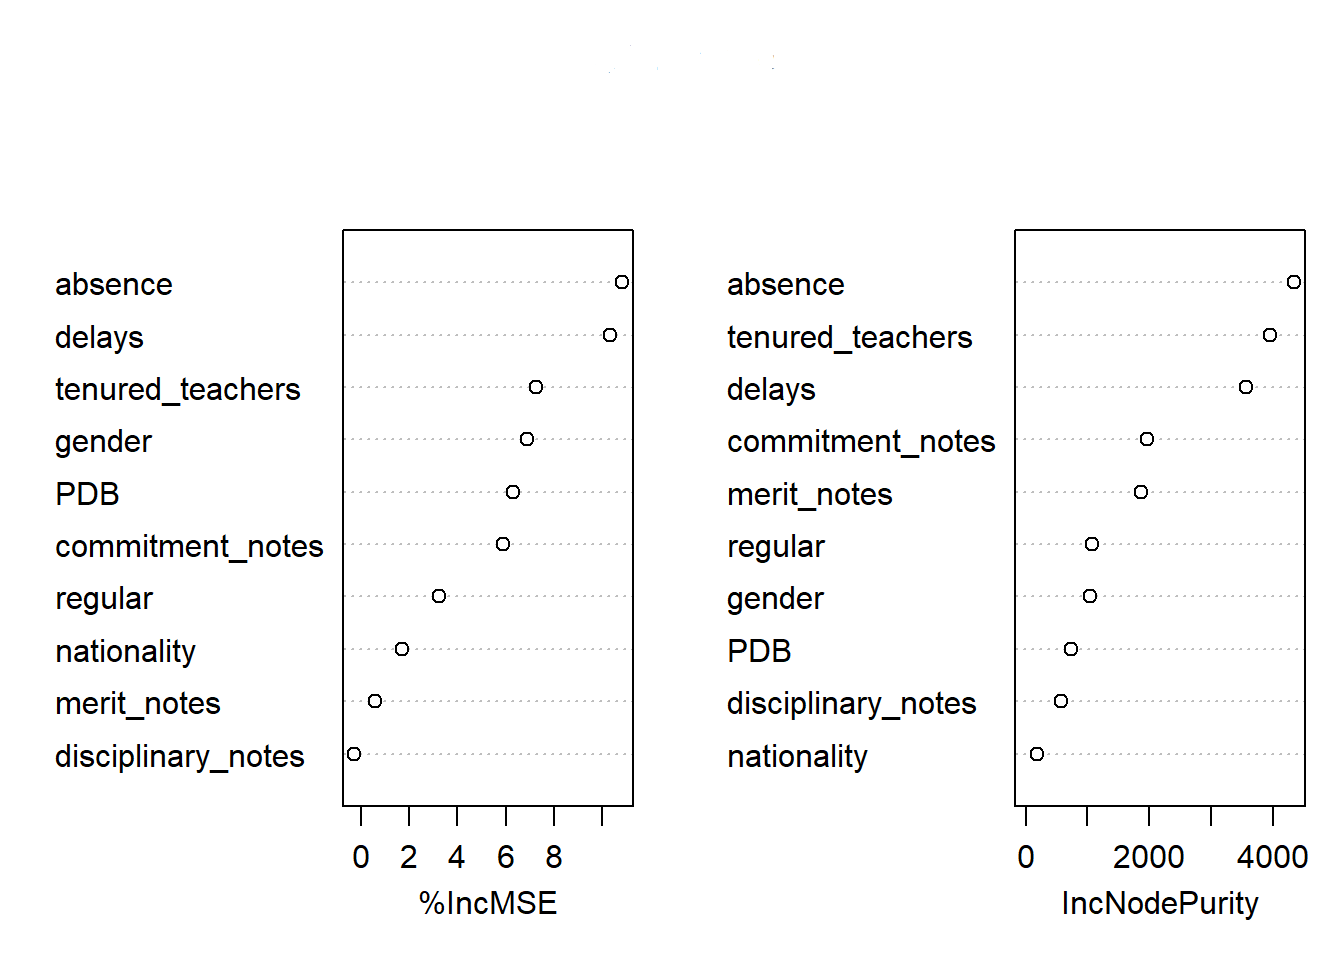
\includegraphics[scale=0.4]{Images/varimp0_2.png}
    }
    \quad
    \subfloat[Variable importance plot of the model with all variables listed in Table \ref{table:fix_var}, excluding \(previous \, math \, grade\).]{
        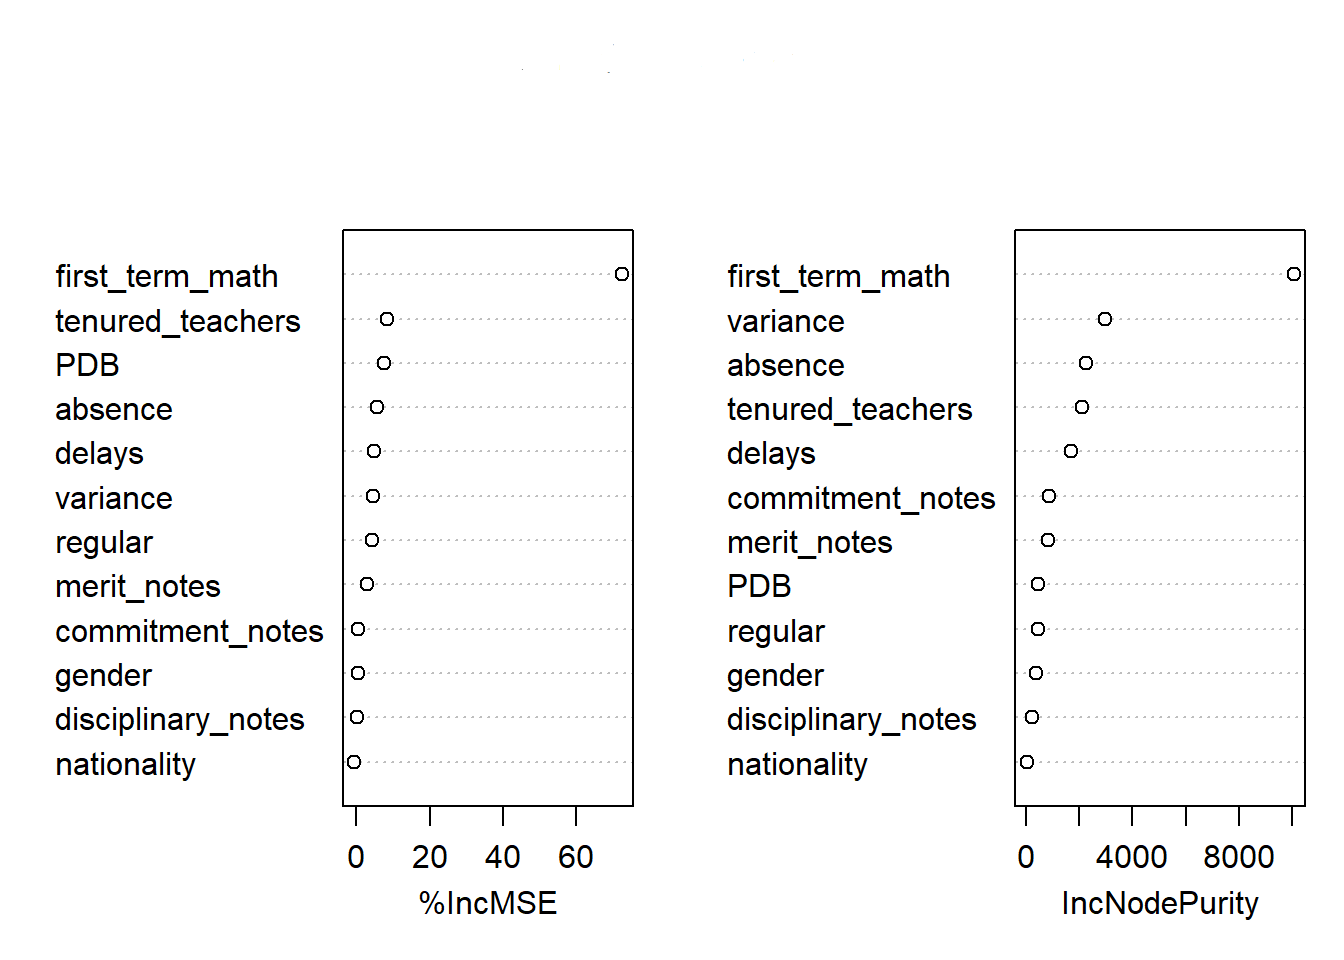
\includegraphics[scale=0.4]{Images/varimp1_2.png}
    }
    \quad
    \subfloat[Variable importance plot of the model with all variables listed in Table \ref{table:fix_var}.]{
        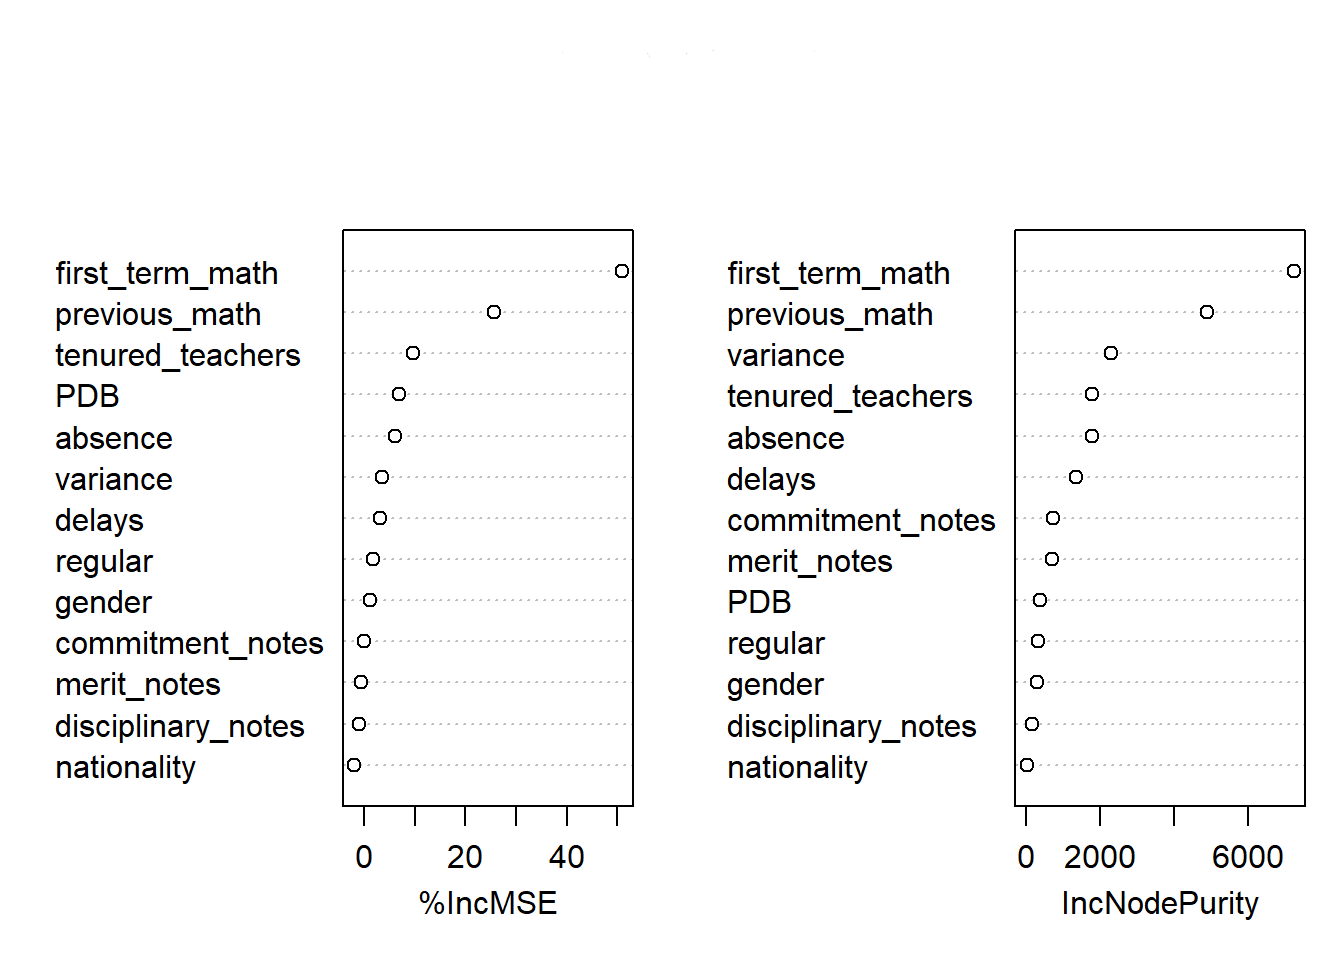
\includegraphics[scale=0.4]{Images/varimp2_2.png}
    }
    \caption[]{Dotcharts of the importance of the fixed variables used in OMERF models in explaining the response.}
    \label{fig:varimp}
\end{figure}

The importance plot for variables identifies significant covariates but does not provide insights into the nature of their relationship with the response variable.
Partial plots, on the other hand, offer a clearer view of how each covariate is associated with the target variable, net to the other covariates included in the model.
Figures \ref{fig:fe0}, \ref{fig:fe1} and \ref{fig:fe2} display partial plots for all continuous and categorical fixed-effect covariates, in each implemented model.

These plots highlight some common patterns: \(absence\) and \(delays\) show an inverse proportional association with the response; on the contrary \(merit \, notes\), \(commitment \, notes\) and obviously \(first \, term \, math\) and \(previous \, math \, grade\) are directly proportional to it;
finally the factor covariates seem to have little to no influence on the target, especially in the last two models.

\begin{figure}[H]
    \centering
    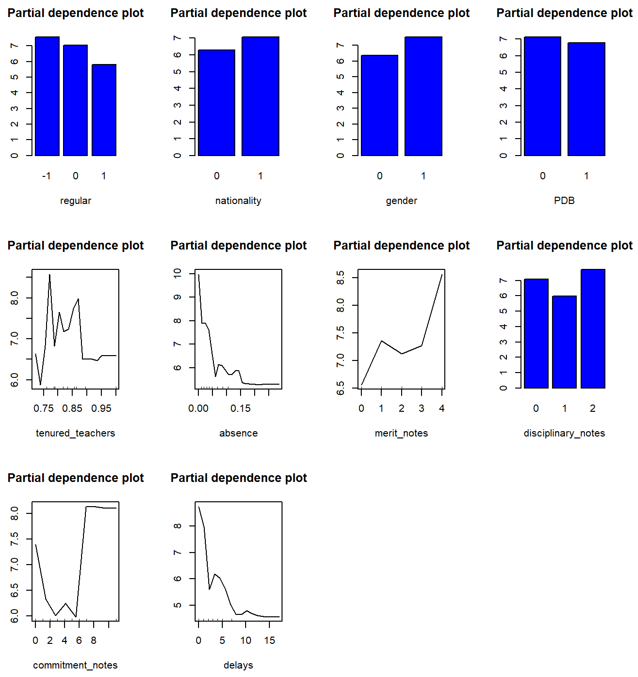
\includegraphics[width=0.61\textwidth]{fe0_2.png}
    \caption{Partial plots of the RF target variable in OMERF method with respect to the covariates of the model with all varaibles listed in Table \ref{table:fix_var}, excluding \(first \, term \, math\), \(variance\), \(previous \, math \, grade\).}
    \label{fig:fe0}
\end{figure}

\begin{figure}[H]
    \centering
    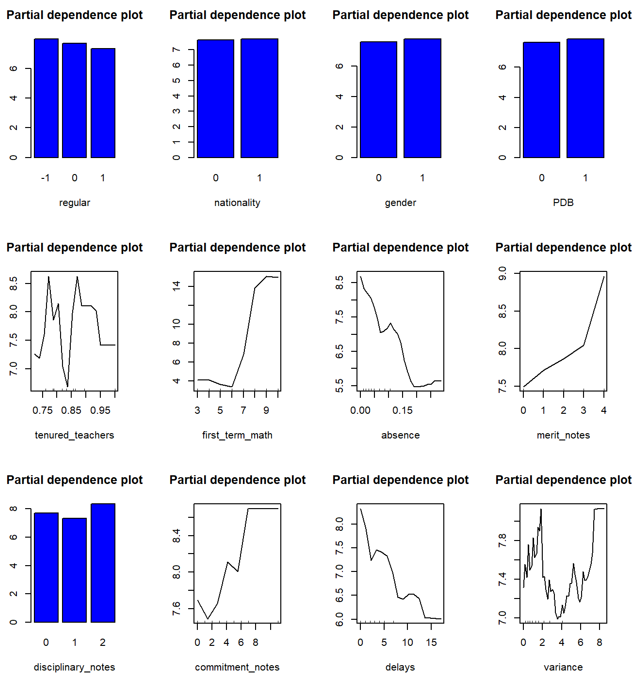
\includegraphics[width=0.61\textwidth]{fe1_2.png}
    \caption{Partial plots of the RF target variable in OMERF method with respect to the covariates of the model with all varaibles listed in Table \ref{table:fix_var}, excluding \(previous \, math \, grade\).}
    \label{fig:fe1}
\end{figure}

\begin{figure}[H]
    \centering
    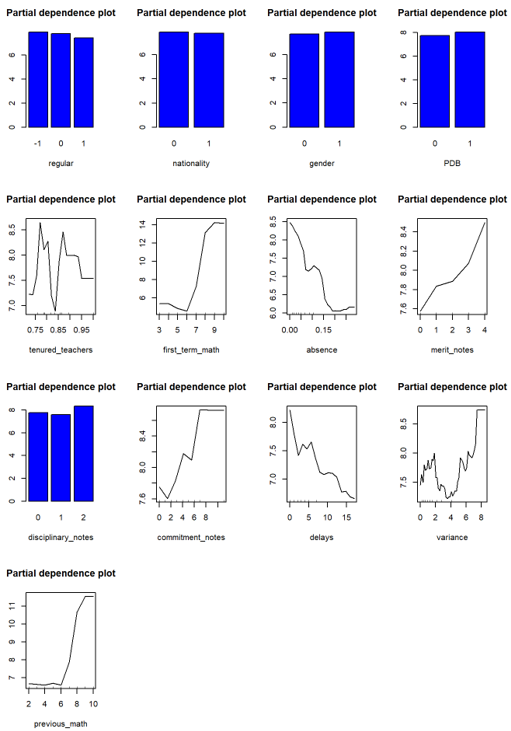
\includegraphics[width=0.61\textwidth]{fe2_2.png}
    \caption{Partial plots of the RF target variable in OMERF method with respect to the covariates of the model with all varaibles listed in Table \ref{table:fix_var}.}
    \label{fig:fe2}
\end{figure}

A potential limitation of the OMERF algorithm stems from the initial step where, during the first initialization, the method estimates the target values (\(\eta_{ijc}\)) through a CLM.
This model imposes a linear effect of covariates on a transformation of the response thereby potentially losing the intricacies that the random forest could capture in the subsequent step of the algorithm.

For this reason a second version of OMERF is implemented, in which the interactions between all covariates and their squares are added to the CLM formula. The resulting performance measures are summarized in Table \ref{table:omerf2}.
The results are better with respect to the previous version and this could be a hint for further developments.

In conclusion, this dataset does not fully justify the use of a method like OMERF, which works more effectively and advantageously in problems with a higher level of complexity.
However, we have received confirmation of how we expected the algorithm to behave, and it is evident that OMERF method is still able to extract additional meaningful insights from the phenomenon under analysis and information on potential nonlinearities.

\begin{table}[H]
    \centering 
    \begin{tabular}{|p{1em} c c c c c c c |}
    \hline
    \rowcolor{bluePoli!40}
    & \textbf{Model} & \textbf{Acc} & \textbf{MSE} & \textbf{ARI} & \textbf{Cohen's k} & \textbf{Cardoso} & \textbf{Ballante} \T\B \\
    \hline \hline
    \textbf{1} & clm & 0.3452 & 2.8571 & 0.0319 & 0.0802 & 0.7309 & 0.2085 \T\B \\
    \textbf{1} & clmm & 0.3690  & $\textcolor{bluePoli}{2.8214}$ & 0.0501 & 0.1121 & 0.7212 & 0.2146 \T\B \\
    \textbf{1} & ordforest & $\textcolor{bluePoli}{0.4405}$ & 43.2738 & $\textcolor{bluePoli}{0.0788}$ & $\textcolor{bluePoli}{0.2229}$ & $\textcolor{bluePoli}{0.6738}$ & $\textcolor{bluePoli}{0.1666}$ \T\B \\
    \textbf{1} & omerf & 0.2976 & 3.3333 & -0.0210 & 0.0012 & 0.7644 & 0.2404 \T\B \\
    \hline
    \textbf{2} & clm & 0.4286 & 1.0238 & 0.1640 & 0.2526 & 0.6096 & 0.1685 \T\B \\
    \textbf{2} & clmm & 0.4286  & $\textcolor{bluePoli}{0.9048}$ & 0.1569 & 0.2532 & $\textcolor{bluePoli}{0.6005}$ & 0.1625 \T\B \\
    \textbf{2} & ordforest & $\textcolor{bluePoli}{0.4762}$ & 36.3929 & $\textcolor{bluePoli}{0.2226}$ & $\textcolor{bluePoli}{0.3046}$ & 0.6021 & $\textcolor{bluePoli}{0.1327}$ \T\B \\
    \textbf{2} & omerf & 0.3571 & 1.9643 & 0.0806 & 0.0836 & 0.6558 & 0.1761 \T\B \\
    \hline
    \textbf{3} & clm & 0.4643 & 0.9167 & 0.1701 & 0.3019 & 0.5839 & 0.1546 \T\B \\
    \textbf{3} & clmm & $\textcolor{bluePoli}{0.5357}$  & $\textcolor{bluePoli}{0.8095}$ & 0.2227 & $\textcolor{bluePoli}{0.3974}$ & $\textcolor{bluePoli}{0.5327}$ & 0.1244 \T\B \\
    \textbf{3} & ordforest & 0.5238 & 36.6429  & $\textcolor{bluePoli}{0.2510}$ & 0.3682 & 0.5563  & $\textcolor{bluePoli}{0.1199}$ \T\B \\
    \textbf{3} & omerf & 0.4048 & 1.7024 & 0.0846 & 0.1559 & 0.6239 & 0.1615 \B \\
    \hline
    \end{tabular}
    \\[10pt]
    \caption{Prediction performances of the four methods in each model listed in Table \ref{table:fix_var}, with ordinal reponse variable the final mathematical grade.}
    \label{table:res_math}
\end{table}


\begin{table}[H]
    \centering 
    \begin{tabular}{|p{1em} c c c c c c c |}
    \hline
    \rowcolor{bluePoli!40}
    & \textbf{Model} & \textbf{Acc} & \textbf{MSE} & \textbf{ARI} & \textbf{Cohen's k} & \textbf{Cardoso} & \textbf{Ballante} \T\B \\
    \hline \hline
    \textbf{4} & clm & 0.4706 & 0.6000 & -0.0065 & -0.0037 & 0.6147 & 0.3859 \T\B \\
    \textbf{4} & clmm & 0.5059 & 0.5294 & -0.0039 & 0.0346 & 0.5688 & 0.3723 \T\B \\
    \textbf{4} & ordforest & $\textcolor{bluePoli}{0.5529}$ & $\textcolor{bluePoli}{0.4471}$ & 0.00002 & 0.1247 & $\textcolor{bluePoli}{0.5212}$ & $\textcolor{bluePoli}{0.2561}$ \T\B \\
    \textbf{4} & omerf & 0.5412 & 0.5294 & $\textcolor{bluePoli}{0.0213}$  & $\textcolor{bluePoli}{0.1487}$ & 0.5609 & 0.3411 \T\B\\
    \hline
    \textbf{5} & clm & 0.6471 & 0.3529 & 0.1326 & 0.3390 & 0.4318 & 0.2309 \T\B \\
    \textbf{5} & clmm & $\textcolor{bluePoli}{0.6588}$ & $\textcolor{bluePoli}{0.3412}$ & $\textcolor{bluePoli}{0.1575}$ & $\textcolor{bluePoli}{0.3647}$ & 0.4259 & 0.2181 \T\B \\
    \textbf{5} & ordforest & $\textcolor{bluePoli}{0.6588}$ & $\textcolor{bluePoli}{0.3412}$ & 0.1263 & 0.3293 & $\textcolor{bluePoli}{0.4128}$ & $\textcolor{bluePoli}{0.1743}$ \T\B \\
    \textbf{5} & omerf & 0.6471 & 0.3529 & 0.1176 & 0.3241 & 0.4361 & 0.2256 \T\B\\
    \hline
    \textbf{6} & clm & 0.7294 & $\textcolor{bluePoli}{0.2706}$ & 0.2925 & 0.4991 & 0.3484 & 0.1808 \T\B \\
    \textbf{6} & clmm & 0.7176 & 0.2824 & 0.2650 & 0.4863 & 0.3689 & $\textcolor{bluePoli}{0.1684}$ \T\B \\
    \textbf{6} & ordforest & 0.7294 & $\textcolor{bluePoli}{0.2706}$ & 0.2686 & 0.4713 & 0.3338 & 0.1812 \T\B \\
    \textbf{6} & omerf & $\textcolor{bluePoli}{0.7529}$ & 0.2824 & $\textcolor{bluePoli}{0.3339}$ & $\textcolor{bluePoli}{0.5193}$ & $\textcolor{bluePoli}{0.3179}$ & 0.1818 \B\\
    \hline
    \end{tabular}
    \\[10pt]
    \caption{Prediction performances of the four methods in each model listed in Table \ref{table:fix_var}, with ordinal reponse variable the created variable \(risk\).}
    \label{table:res_risk}
\end{table}

\begin{table}[H]
    \centering 
    \begin{tabular}{|p{1em} c c c c c c c |}
    \hline
    \rowcolor{bluePoli!40}
    & \textbf{Model} & \textbf{Acc} & \textbf{MSE} & \textbf{ARI} & \textbf{Cohen's k} & \textbf{Cardoso} & \textbf{Ballante} \T\B \\
    \hline \hline
    \textbf{4} & omerf new & 0.5529 & 0.6588 &  0.0719 & 0.2444 & 0.5755 & 0.3320 \T\B \\
    \hline
    \textbf{5} & omerf new & 0.6824 & 0.3176 & 0.1998 & 0.4219 & 0.4144 & 0.2013 \T\B \\
    \hline
    \textbf{6} & omerf new & 0.7176 & 0.2824 & 0.2536 & 0.4842 & 0.3737 & 0.1722 \B \\
    \hline
    \end{tabular}
    \\[10pt]
    \caption{Prediction performances of the new version of OMERF method in each model listed in Table \ref{table:fix_var}, with ordinal reponse variable the created variable \(risk\).}
    \label{table:omerf2}
\end{table}




%-----------------------------------------------------------------------------
% CONCLUSION
%-----------------------------------------------------------------------------
\section{Conclusions}
\label{sec:conclusions}
\color{black}
In this work, a method called Ordinal Mixed-Effects Random Forest (OMERF) is introduced. 
This approach innovatively extends the application of random forest to the analysis of hierarchical data, specifically for ordinal response variables.
The OMERF model replaces the linear combination of fixed-effect covariates in a cumulative linear mixed model with a random forest.
This novel approach makes a valuable contribution to the statistical literature on aggregated models combining mixed-effects models and tree-based methods.
It inherits the flexibility and predictive power of random forests while preserving the structure of mixed-effects models for ordinal response.

To show the performance of the proposed model simulation study is performed. Subsequently, OMERF algorithm is applied to a real world dataset containing  all the personal information stored in the school's electronic register of a prestigious high school in Milan, in order to identify students who may be at risk of failure and generally of predicting their academic progress.

In the simulation study, the performance of the proposed mixed-effects tree-based method was a clear improvement compared to CLM and CLMM models when the data generating process features nonlinear patterns.
In addition, the predictive power of the OMERF model was comparable to the one of the ordinal random forest model.
Overall, the main advantages of the OMERF algorithm are its flexibility and data inspection capability.
By relaxing the linear assumption of the fixed-effects part, the method could model more complex functional forms, detecting also potential interactions
among covariates, for both categorical and continuous variables.

For this reason, the decision to use OMERF over CLMM depends on the complexity of the fixed effects structure, which is often not known in advance.
If fixed-effect covariates exhibit a linear association with the response and are not correlated, CLMM is expected to perform better.
Conversely, if the covariate set is large, and the covariates potentially interact, creating complex patterns in their association with the response, OMERF is expected to outperform parametric methods with predefined functional forms.
At the same time, when data present a hierarchy, the method is able to take into account the dependence structure within observations and to model it.
In the educational data mining context, this aspect is essential in order to better understand students and the settings in which they learn.

In conclusion, OMERF proves to be a powerful and an easily interpretable method, that can deal with a grouped data structure and can be applied to various complex real data challenges.

In the case study, we give a contribution to the learning analytics area. OMERF method, when applied to educational data, can be a useful tool to support the definition of best practices and
new tutoring programmes aimed at enhancing student performances and helping students at risk. 


However, a potential limitation of the OMERF algorithm stems from the initial step where, during the first initialization, the method estimates the target values (\(\eta_{ijc}\)) through a CLM.
This model imposes a linear effect of covariates on a transformation of the response thereby potentially losing the intricacies that the random forest could capture in the subsequent step of the algorithm.
Therefore, a hint for further developments might be to consider using a different model that can successfully capture nonlinear relationships and interactions between covariates and help initialize the \(\eta_{ijc}\) estimates, thereby allowing the OMERF method to perform at its best.




%-----------------------------------------------------------------------------
% BIBLIOGRAPHY
%-----------------------------------------------------------------------------
\bibliography{bibliography.bib}

\appendix
\section{Appendix A}
\label{sec:appA}

\begin{lstlisting}[language=R]
  omerf= function (y, cov, group, xnam=NULL, znam=NULL, bizero=NULL, 
                 itmax=100, toll=0.05) {
  #ordinal mixed-effects random forest (OMERF)
  #inputs: 
  #-y = vector of responses
  #-cov = data frame with all the fixed covariates for each statistical unit
  #-group = factor vector which, for each statistical unit,
  #         tells the group to which it belongs (random effect)
  #-xnam = vector with the names of the fixed covariates 
  #        to be used in the random forest
  #-znam = vector with the names of the covariates
  #        to be used in the random effects
  #-bizero = matrix containing the coefficients of the random effects
  #          (the first value of each column is the intercept,
  #           the other ones are the covariates znam)
  # assume that group and bizero are coherent, ie b[,i] 
  # corresponds to levels(group)[i]
  
  ###### STEP 1: Initialization  ######

  N <- length(y) #number of observations
  n=length(levels(group)) #number of groups
  
  q <- length(znam)+1	#number of random covariates + random intercept
  Zi=NULL
  z.not.null=!(is.null(znam)) #check whether there are 
                              #covariates included in the random effects
  if (z.not.null) Zi=cov[znam] #random effects covariates
  Zi.int= cbind(rep(1,N),Zi) #random intercept + random effects covariates
  
  #Initialize (if NULL) bi to 0
  if( is.null(bizero) ){
    bi <- NULL
    for(i in 1:n) bi=cbind(bi,rep(0,q))
  }	
  if( !is.null(bizero) ) bi=bizero
  lev=levels(group) #group names
  bi=data.frame(bi)
  names(bi)=lev
  all.bi=list()  #bi of each iteration
  all.bi[[1]]=bi
  
  #if xnam is NULL assume that all cov variables are to be used
  if(is.null(xnam)) xnam=names(cov)
  
  #group must be a factor, otherwise it gives an error
  if(!is.factor(group)) stop("The "group" argument must be a factor")
  
  forest.formula=as.formula(paste("target~", paste(xnam, collapse= "+")))
  
  if(z.not.null) {
    clmm.formula=as.formula(paste("y~offset(f.x_ij)+(1+", 
    paste(znam, collapse= "+"), "|group)"))
  }
  else {clmm.formula=as.formula(paste("y~offset(f.x_ij)+(1|group)"))}
  


  ###### STEP 2: CLM for mu_ij initialization ######

  library(ordinal)
  clm.formula=as.formula(paste("y~", paste(xnam, collapse= "+")))
  clm.data= cbind(y,cov[xnam])
  clm.0=clm(clm.formula, data=clm.data, link="logit")
  mu.ij.0=clm.0$fitted.values #P(yij=c)
  prob.est=predict(clm.0,clm.data,type = "cum.prob")[1]$cprob1
  prob.est[which(prob.est==1)]=0.99999999
  eta.est=qlogis(prob.est) #linear predictor of clm
  
  ###### STEP 3-4: Iterative model estimation  ######

  library(randomForest)
  it=1
  converged=FALSE
  while(!converged && it<itmax) {
    
    #random forest
    target=rep(0,N) #target=eta+Z%*%b
    for (i in 1:N) {
      b.temp=as.matrix(bi[group[i]], nrow=q, ncol=1)
      z.temp=as.matrix(Zi.int[i,], nrow=1, ncol=q)
      target[i]= eta.est[i] + z.temp%*%b.temp
    }
    forest.data=cbind(target, cov[xnam])
    forest=randomForest(forest.formula, forest.data, importance=TRUE) 
    f.x_ij=forest$predicted
    
    clmm.data = data.frame(y,cov[znam],group,f.x_ij)
    
    clmm.fit= clmm(clmm.formula, link="logit", data=clmm.data, Hess=TRUE, 
    control=clmm.control(maxLineIter = 500, maxIter=1000, grtol=1e-3))
    
    #I want to maintain the order of the elements of bi
    select=c("(Intercept)",znam) #all bi to be extracted
    clmm.bi=ranef(clmm.fit)$group[select]
    
    #convergence of bi
    bi.old=bi
    bi=data.frame(t(clmm.bi))
    names(bi)=lev
    diff.t=abs(bi.old-bi)
    n.diff=max(diff.t) #use the infinite norm (max)
    ind=which(diff.t==n.diff, arr.ind=T)
    n.old=abs(bi.old[ind])
    converged= n.diff/n.old <toll
    
    it=it+1
    all.bi[[it]]=bi
  }
 
  ###### STEP 5: Output preparation  ######

  #if there is no convergence it gives an error message
  if(!converged) {
    warning("Maximum number of iterations exceeded, no convergence achieved")
  }
  result=list(clmm.fit,forest,target,bi,it,converged,all.bi,xnam)
  names(result)=c("clmm.model", "forest.model","rf.target",
                  "rand.coef", "n.iteration","converged",
                  "all.rand.coef","forest.var")
  class(result)="omerf"
  result
}


###### Auxiliary functions  ######


summary.omerf=function(om) {
  print("Mixed effects model") #summary of the mixed effects model
  print(summary(om$clmm.model)) 
  str=ifelse(om$converged, "Converged", "Did not converge")
  print(paste(str , "after", om$n.iteration, "iterations"))
  #says whether there is convergence
}


fitted.omerf=function(om, group, type="response") {
  #the correct fitted values are already those of the clmm function,
  #as they incorporate the fitted values of the random forest into the model
  mu_avg=om$clmm.model$fitted.values #for an avg random effect
  f.x_ij=om$forest.model$predicted
  y_train=as.numeric(om$clmm.model$y)
  
  ranef=rowSums(ranef(om$clmm.model)$gr)
  mu=rep(0,length(mu_avg))
  eta=rep(0,length(mu_avg))
  for (j in 1:length(mu_avg)) {
    i=group[j]
    c=y_train[j]-min(y_train)+1
    if(c==1) {
      eta[j]=om$clmm.model$Theta[c] - ranef[i] - f.x_ij[j]
      mu[j]=plogis(eta[j])
    } else if(c==max(y_train)-min(y_train)+1) {
      eta[j]=qlogis(0.99999999)
      mu[j]=1 - plogis(om$clmm.model$Theta[c-1] - ranef[i] - f.x_ij[j])
      # 1 - P(yij<=c-1)
    } else {
      eta[j]=om$clmm.model$Theta[c] - ranef[i] - f.x_ij[j]
      mu[j]=plogis(eta[j]) - 
        plogis(om$clmm.model$Theta[c-1] - ranef[i] - f.x_ij[j])
        # P(yij<=c) - P(yij<=c-1)
    }
  }
  #error if the answer type is not one of the following
  allowed=c("response", "mu", "eta")
  msg=paste("Possible choices are", allowed[1],"," ,allowed[2],"and", 
            allowed[3], sep="")
  if(sum(type==allowed)==0) stop("Type of prediction not available:",msg)
  if(type=="mu") ans=mu # P(yij=c)
  if(type=="response") ans=as.factor(y_train)
  if(type=="eta") ans=eta
  ans
}






predict.omerf=function(om, y_train, newdata, group, type="response", 
                       predict.all=FALSE) {
  forest.data=newdata[om$forest.var]		
  f.x_ij=predict(om$forest.model,forest.data,predict.all=predict.all)
  
  preds <- as.data.frame(matrix(0, dim(newdata)[1], length(levels(y_train))))
  eta <- as.data.frame(matrix(0, dim(newdata)[1], length(levels(y_train))))
  ranef=rowSums(ranef(om$clmm.model)$group)
  lev=levels(y_train)
  names(preds) = lev
  names(eta) = lev
  for (c in 1:length(lev)) {
    for (j in 1:dim(newdata)[1]) {
      i=group[j]
      if(c==1) {
        eta[j,c]=om$clmm.model$Theta[c] - ranef[i] - f.x_ij[j]
        preds[j,c]=plogis(eta[j,c])
      } else if(c==length(lev)) {
        eta[j,c]=qlogis(0.99999999)
        preds[j,c]=1 - plogis(om$clmm.model$Theta[c-1] - ranef[i] - f.x_ij[j])
        # 1 - P(yij<=c-1)
      } else {
        eta[j,c]=om$clmm.model$Theta[c] - ranef[i] - f.x_ij[j]
        preds[j,c]=plogis(eta[j,c]) - 
          plogis(om$clmm.model$Theta[c-1] - ranef[i] - f.x_ij[j])
          # P(yij<=c) - P(yij<=c-1)
      }
    }
  }
  max_mu <- apply(preds, 1, max)
  pred_val <- names(preds)[apply(preds, 1, which.max)]
  
  
  #error if the answer type is not one of the following
  allowed=c("response", "mu", "eta")
  msg=paste("Possible choices are", allowed[1],"," ,allowed[2],"and", 
            allowed[3], sep="")
  if(sum(type==allowed)==0) stop("Type of prediction not available:",msg)
  
  if(type=="eta") ans=eta # eta for the predicted class
  if(type=="mu") ans=preds # P(yij=c) c=1,...,C
  if(type=="response") ans=pred_val
  ans
}


ranef.omerf=function(om, group, znam=NULL) {
  ranef=ranef(om$clmm.model)$gr
  n = (length(znam)+1)*length(levels(group))
  step = length(levels(group))
  par(mfrow=c(1,length(znam)+1))
  for (i in 1:(length(znam)+1)) {
    condVar=rep(0,step)
    if(is.null(znam)) { condVar_temp = om$clmm.model$condVar
    } else { condVar_temp = om$clmm.model$condVar[((i - 1) * step + 1):(i * step),((i - 1) * step + 1):(i * step)] }
    for (l in 1:step) {
      if(is.null(znam)) { 
         condVar[l] <- condVar_temp[l]
      } else {condVar[l] <- condVar_temp[l,l]}
    }
    condVar_sqrt <- sqrt(condVar)
    ci <- ranef[,i] + qnorm(0.975) * condVar_sqrt %o% c(-1, 1)
    ord.re <- order(ranef[,i])
    lev <- levels(group)
    ci <- ci[order(ranef[,i]),]
    plot(1:length(lev), ranef[ord.re,i], axes=FALSE, ylim=range(ci),
         xlab="random variable", ylab="random effect")
    axis(1, at=1:length(lev), labels = lev[ord.re])
    axis(2)
    for(k in 1:length(lev)) segments(k, ci[k,1], k, ci[k, 2])
    abline(h = 0, lty=2)
  }
}


  
\end{lstlisting}
%
\section{Appendix B}
It may be necessary to include another appendix to better organize the presentation of supplementary material.


% @article{knuth74,
%     author = {Knuth, Donald E.},
%     title = {Computer Programming As an Art},
%     journal = {Commun. ACM},
%     year = {1974},
%     pages = {667--673},
%     numpages = {7},
%     publisher = {ACM},
%     address = {New York, NY, USA}
% }

% @article{knuth92,
%     author = {Knuth, Donald E.},
%     title = {Two notes on notation},
%     journal = {Amer. Math. Monthly},
%     volume = {99},
%     year = {1992},
%     pages = {403--422}
% }

% @book{lamport94,
%     title = {LaTeX: A Document Preparation System},
%     author = {Lamport, Leslie},
%     year = {1994},
%     publisher = {Pearson Education India}
% }

% @article{article,
%   author  = {Peter Adams}, 
%   title   = {The title of the work},
%   journal = {The name of the journal},
%   year    = 1993,
%   number  = 2,
%   pages   = {201-213},
%   month   = 7,
%   note    = {An optional note}, 
%   volume  = 4
% }

% @book{book,
%   author    = {Peter Babington}, 
%   title     = {The title of the work},
%   publisher = {The name of the publisher},
%   year      = 1993,
%   volume    = 4,
%   series    = 10,
%   address   = {The address},
%   edition   = 3,
%   month     = 7,
%   note      = {An optional note},
%   isbn      = {3257227892}
% }

% @booklet{booklet,
%   title        = {The title of the work},
%   author       = {Peter Caxton}, 
%   howpublished = {How it was published},
%   address      = {The address of the publisher},
%   month        = 7,
%   year         = 1993,
%   note         = {An optional note}
% }

% @conference{conference,
%   author       = {Peter Draper}, 
%   title        = {The title of the work},
%   booktitle    = {The title of the book},
%   year         = 1993,
%   editor       = {The editor},
%   volume       = 4,
%   series       = 5,
%   pages        = 213,
%   address      = {The address of the publisher},
%   month        = 7,
%   organization = {The organization},
%   publisher    = {The publisher},
%   note         = {An optional note}  
% }

% @inbook{inbook,
%   author       = {Peter Eston}, 
%   title        = {The title of the work},
%   chapter      = 8,
%   pages        = {201-213},
%   publisher    = {The name of the publisher},
%   year         = 1993,
%   volume       = 4,
%   series       = 5,
%   address      = {The address of the publisher},
%   edition      = 3,
%   month        = 7,
%   note         = {An optional note}
% }

% @incollection{incollection,
%   author       = {Peter Farindon}, 
%   title        = {The title of the work},
%   booktitle    = {The title of the book},
%   publisher    = {The name of the publisher},
%   year         = 1993,
%   editor       = {The editor},
%   volume       = 4,
%   series       = 5,
%   chapter      = 8,
%   pages        = {201-213},
%   address      = {The address of the publisher},
%   edition      = 3,
%   month        = 7,
%   note         = {An optional note}
% }

% @manual{manual,
%   title        = {The title of the work},
%   author       = {Peter Gainsford}, 
%   organization = {The organization},
%   address      = {The address of the publisher},
%   edition      = 3,
%   month        = 7,
%   year         = 1993,
%   note         = {An optional note}
% }

% @mastersthesis{mastersthesis,
%   author       = {Peter Harwood}, 
%   title        = {The title of the work},
%   school       = {The school of the thesis},
%   year         = 1993,
%   address      = {The address of the publisher},
%   month        = 7,
%   note         = {An optional note}
% }

% @misc{misc,
%   author       = {Peter Isley}, 
%   title        = {The title of the work},
%   howpublished = {How it was published},
%   month        = 7,
%   year         = 1993,
%   note         = {An optional note}
% }

% @phdthesis{phdthesis,
%   author       = {Peter Joslin}, 
%   title        = {The title of the work},
%   school       = {The school of the thesis},
%   year         = 1993,
%   address      = {The address of the publisher},
%   month        = 7,
%   note         = {An optional note}
% }

% @proceedings{proceedings,
%   title        = {The title of the work},
%   year         = 1993,
%   editor       = {Peter Kidwelly},
%   volume       = 4,
%   series       = 5,
%   address      = {The address of the publisher},
%   month        = 7,
%   organization = {The organization},
%   publisher    = {The name of the publisher},
%   note         = {An optional note}
% }

% @techreport{techreport,
%   author       = {Peter Lambert}, 
%   title        = {The title of the work},
%   institution  = {The institution that published},
%   year         = 1993,
%   number       = 2,
%   address      = {The address of the publisher},
%   month        = 7,
%   note         = {An optional note}
% }

% @unpublished{unpublished,
%   author       = {Peter Marcheford}, 
%   title        = {The title of the work},
%   note         = {An optional note},
%   month        = 7,
%   year         = 1993
% }

% @online{online,
%   author       = {MultiMedia LLC}, 
%   title        = {{MS Windows NT} Kernel Description},
%   year         = 1999,
%   url          = {http://www.whateveritis.com},
%   urldate      = {2010-09-30}
% }

% @patent{edison,
%     title      = {Electric distribution system},
%     author     = {Edison, Thomas A.},
%     number     = {266793},
%     type       = {patentus},
%     date       = {1882-10-31}
% }

% @article{oetiker1995not,
%   title={The not so short introduction to LATEX2$\varepsilon$},
%   author={Oetiker, Tobias and Partl, Hubert and Hyna, Irene and Schlegl, Elisabeth},
%   journal={Electronic document available at http://www. tex. ac. uk/tex-archive/info/lshort},
%   year={1995},
%   publisher={Citeseer}
% }

% @book{kottwitz2015latex,
%   title={LaTeX Cookbook},
%   author={Kottwitz, Stefan},
%   year={2015},
%   publisher={Packt Publishing Ltd}
% }

% @misc{bibtex,
%   author       = {CTAN}, 
%   title        = {{B}i{B}{T}e{X} Documentation},
%   url          = {https://ctan.org/topic/bibtex-doc}
% }

% @misc{tikz,
%   author       = {CTAN}, 
%   title        = {pgf – Create {P}ost{S}cript and {PDF} graphics in {TEX}},
%   url          = {https://www.ctan.org/pkg/pgf}
% }

%%%%%%%%%%%%%%%%%%%%%%%%%%%%%%%%%%%%%%%%%%%%%%%%%%%%%%%%%%%%%%
%%     ABSTRACT IN ITALIAN LANGUAGE AND ACKNOWLEDGMENTS     %%
%%%%%%%%%%%%%%%%%%%%%%%%%%%%%%%%%%%%%%%%%%%%%%%%%%%%%%%%%%%%%%
\cleardoublepage

%-----------------------------------------------------------------------------
% SOMMARIO
%-----------------------------------------------------------------------------
\section*{Abstract in lingua italiana}
In questa tesi, proponiamo un innovativo metodo statistico. Il modello è chiamato Ordinal Mixed-Effect Random Forest (OMERF) e estende l'uso delle random forest all'analisi di dati gerarchici per modellare risposte categoriche ordinali.
Questo metodo preserva la flessibilità e la capacità di modellare strutture complesse sia per variabili categoriche che continue, tipiche dei metodi ensemble ad albero.
Allo stesso tempo, il modello OMERF tiene conto della struttura nidificata dei dati gerarchici, modellando la dipendenza che esiste al livello più alto della gerarchia e consentendo l'inferenza statistica su questa struttura.
In questo studio, è stata condotta una simulazione per validare le prestazioni del metodo proposto e confrontarlo con i più noti modelli già esistenti.
L'utilizzo dell'algoritmo OMERF è esemplificato dall'applicazione ad un caso reale incentrato sulla modellazione degli studenti a rischio di insuccesso di una prestigiosa scuola superiore di Milano e sulla previsione dei loro progressi accademici.
Il modello è in grado di identificare le caratteristiche discriminanti degli studenti e stimare l'effetto di ciascuna classe a cui gli studenti appartengono.
\vspace{15pt}
\begin{tcolorbox}[arc=0pt, boxrule=0pt, colback=bluePoli!60, width=\textwidth, colupper=white]
    \textbf{Parole chiave:} risposta ordinale, dati gerarchici, random forest, modelli a effetti misti, learning analytics 
\end{tcolorbox}

%-----------------------------------------------------------------------------
% ACKNOWLEDGEMENTS
%-----------------------------------------------------------------------------
\section*{Ringraziamenti}

Desidero esprimere la mia gratitudine alla relatrice di questa tesi, la professoressa Chiara Masci, per avermi offerto l'opportunità di contribuire a questo progetto di ricerca e per il suo continuo sostegno e incoraggiamento.
Un ringraziamento speciale è rivolto anche alla correlatrice Lidia Rossi, per la sua generosa disponibilità e per il suo costante supporto. \medskip

Ringrazio infinitamente i miei genitori e mio fratello, perchè mi hanno sempre motivato a dare il meglio, per il loro affetto e per la loro comprensione durante questo intenso periodo di studio. \medskip

Un grazie alle mie amiche più care, Chiara, Marzia, Rebecca e Beatrice, che hanno alleggerito i momenti più pesanti e mi sono sempre state vicine. \medskip

Infine, sono profondamente grata di aver incontrato tante persone che sono diventate amiche durante il mio percorso universitario. Insieme, abbiamo condiviso tanti ricordi e ci siamo supportati nei momenti più impegnativi. In particolare, grazie a Chiara e Michela per la vostra preziosa amicizia.


%-------------------------------------------------------------------------
%	END OF YOUR DOCUMENT
%-------------------------------------------------------------------------
\end{document}